%%
%% Copyright 2019-2024 Elsevier Ltd
%%
%% This file is part of the 'CAS Bundle'.
%% --------------------------------------
%%
%% It may be distributed under the conditions of the LaTeX Project Public
%% License, either version 1.3c of this license or (at your option) any
%% later version.  The latest version of this license is in
%%    http://www.latex-project.org/lppl.txt
%% and version 1.3c or later is part of all distributions of LaTeX
%% version 1999/12/01 or later.
%%
%% The list of all files belonging to the 'CAS Bundle' is
%% given in the file `manifest.txt'.
%%
%% Template article for cas-sc documentclass for
%% double column output.


\documentclass[a4paper,fleqn]{cas-sc}

% If the frontmatter runs over more than one page
% use the longmktitle option.

%\documentclass[a4paper,fleqn,longmktitle]{cas-sc}

%\usepackage[numbers]{natbib}
%\usepackage[authoryear]{natbib}
\usepackage[numbers,sort&compress]{natbib}

%%%Author macros
\def\tsc#1{\csdef{#1}{\textsc{\lowercase{#1}}\xspace}}
\tsc{WGM}
\tsc{QE}
%%%

% Uncomment and use as if needed
%\newtheorem{theorem}{Theorem}
%\newtheorem{lemma}[theorem]{Lemma}
%\newdefinition{rmk}{Remark}
%\newproof{pf}{Proof}
%\newproof{pot}{Proof of Theorem \ref{thm}}

\usepackage{amsmath,amssymb}
\usepackage{graphicx}
\usepackage{booktabs}
\usepackage{float}
\usepackage{amsmath,amssymb}
\usepackage{tikz}
\usetikzlibrary{positioning,arrows.meta,calc,fit,backgrounds}
\newtheorem{theorem}{Theorem}
\newtheorem{proposition}[theorem]{Proposition}
\newtheorem{lemma}[theorem]{Lemma}
\newdefinition{remark}{Remark}
\newproof{proof}{Proof}

\begin{document}
\let\WriteBookmarks\relax
\def\floatpagepagefraction{1}
\def\textpagefraction{.001}

% Short title
\shorttitle{}

% Short author
\shortauthors{}

% Main title of the paper
\title [mode = title]{An all-Mach IMEX scheme for the six-equation two-phase model with unified mechanical, thermal and chemical relaxation at arbitrary rates}

% Title footnote mark
% eg: \tnotemark[1]
\tnotemark[1]

% Title footnote 1.
% eg: \tnotetext[1]{Title footnote text}
\tnotetext[1]{}

% First author
%
% Options: Use if required
% eg: \author[1,3]{Author Name}[type=editor,
%       style=chinese,
%       auid=000,
%       bioid=1,
%       prefix=Sir,
%       orcid=0000-0000-0000-0000,
%       facebook=<facebook id>,
%       twitter=<twitter id>,
%       linkedin=<linkedin id>,
%       gplus=<gplus id>]

\author[1]{}%[<options>]

% Corresponding author indication
\cormark[1]

% Footnote of the first author
\fnmark[1]

% Email id of the first author
\ead{}

% URL of the first author
\ead[url]{}

% Credit authorship
% eg: \credit{Conceptualization of this study, Methodology, Software}
\credit{}

% Address/affiliation
\affiliation[1]{organization={},
            addressline={},
            city={},
%          citysep={}, % Uncomment if no comma needed between city and postcode
            postcode={},
            state={},
            country={}}

\author[2]{}%[]

% Footnote of the second author
\fnmark[2]

% Email id of the second author
\ead{}

% URL of the second author
\ead[url]{}

% Credit authorship
\credit{}

% Address/affiliation
\affiliation[2]{organization={},
            addressline={},
            city={},
%          citysep={}, % Uncomment if no comma needed between city and postcode
            postcode={},
            state={},
            country={}}

% Corresponding author text
\cortext[1]{Corresponding author}

% Footnote text
\fntext[1]{}

% For a title note without a number/mark
%\nonumnote{}

% Here goes the abstract
\begin{abstract}
We present a second-order semi-implicit finite volume scheme for the single-velocity six-equation two-phase model
with total energy, for stiffened-gas and Noble--Abel stiffened-gas phases with mechanical, thermal and chemical
relaxation and for Mie--Gr\"uneisen phases with instantaneous mechanical relaxation. The acoustic waves at low Mach
numbers and the relaxation up to infinite rates are treated in a single implicit step: the pressure work and the three
relaxation processes, a slower process being active only when the faster ones are instantaneous, enter one local
closure per cell, solved by scalar root finding, and each stage requires a Newton solve of a nonlinear system for the
cell pressures, with a time step restricted by the flow velocity only. At fixed mesh, under non-degeneracy
assumptions and for data on the equilibrium manifold, the scheme converges to the corresponding equilibrium schemes as the relaxation rates tend to infinity,
and it is formally asymptotic preserving in the low Mach number limit. At shocks, the defect between the conservative
and non-conservative mixture internal energies is shared between the phases according to the shock relations of the
model, uniquely for weak shocks and by shooting for strong ones, without calibrated heat exchange. All quantities are
transported explicitly by a path-conservative Rusanov scheme with the material speed, and the implicit acoustic
dissipation vanishes at low Mach numbers. A stiffly accurate implicit--explicit (IMEX) Runge--Kutta scheme gives
second order in time. We prove that the scheme preserves moving contacts between stiffened-gas or Noble--Abel
stiffened-gas phases, at uniform temperature when thermal or chemical relaxation is active. Numerical results in one
and two dimensions, from the incompressible limit to strong shocks, cavitation and phase transition, confirm the
accuracy and robustness of the method.
\end{abstract}


% Use if graphical abstract is present
%\begin{graphicalabstract}
%\includegraphics{}
%\end{graphicalabstract}

% Research highlights
\begin{highlights}
\item
\item
\item
\end{highlights}


% Keywords
% Each keyword is seperated by \sep
\begin{keywords}
Compressible two-phase flows \sep
Phase transition \sep
Six-equation model \sep
Relaxation processes\sep
All Mach number IMEX scheme \sep
Asymptotic preserving \sep
Well-balanced \sep
 \sep \sep \sep
\end{keywords}

\maketitle

% =====================================================================
% Section 1. Introduction
% =====================================================================
\section{Introduction}
\label{sec:intro}

The single-velocity six-equation two-phase model with relaxation \cite{SPB2009,PelantiShyue2014,Pelanti2022} is widely
used for compressible liquid--gas and liquid--vapour flows: cavitation in hydraulic machinery and fuel injectors,
flashing and evaporation fronts and the rapid depressurisation of pressurised water in nuclear reactor safety,
underwater explosions, and the shock loading of condensed materials and mixtures
\cite{SaurelPetitpasAbgrall2008,Bartak1990,PelantiShyue2019,Chiapolino2017,DeLorenzo2018,DeLorenzo2019,Schmidmayer2020,SaurelPantano2018}.
Two features make these flows difficult. First, the Mach number varies by orders of magnitude within one flow: a slowly moving liquid is in the incompressible regime, while gas, vapour pockets or detonation products may be
transonic or carry strong shocks. Second, the phases exchange momentum, heat and mass on time scales from much slower to
much faster than the flow, so that one computation contains frozen, finite-rate and equilibrium regions, and phase
transition through metastable states.

Diffuse-interface models describe pure fluids, interfaces and mixtures with one set of equations throughout the domain
\cite{SaurelAbgrall1999a,AbgrallKarni2001,SaurelPantano2018}. They derive from the Baer--Nunziato seven-equation model
\cite{BaerNunziato1986}, where each phase has its own velocity and pressure. Velocity relaxation gives the two-pressure
six-equation model, additional pressure relaxation the five-equation model of Kapila et al.\
\cite{Kapila2001,MurroneGuillard2005,AllaireClercKokh2002}, and further thermal and chemical relaxation the
four-equation $pT$ model and the homogeneous equilibrium model \cite{FlattenLund2011,Lund2012,Pelanti2022}. Saurel,
Petitpas and Berry \cite{SPB2009} proposed computing interfaces and mixtures with the six-equation model and stiff
pressure relaxation: its frozen sound speed is monotone in the volume fraction, its volume-fraction equation contains
only the pressure work, and the mixture total energy, redundant for smooth flows, is added as a seventh, ``+1'' equation
to recover the conservative mixture energy at shocks. Pelanti and Shyue \cite{PelantiShyue2014} made the approach
mixture-energy consistent and added heat and mass transfer \cite{SaurelPetitpasAbgrall2008,Zein2010}, and Pelanti
\cite{Pelanti2022} extended the relaxation procedures to arbitrary rates and to the Noble--Abel stiffened-gas
\cite{LeMetayerSaurel2016} and Mie--Gr\"uneisen equations of state.

A known difficulty of the six-equation model is its behaviour at shocks in mixtures: the model is non-conservative, its
shock relations \cite{SaurelGavrilyukRenaud2003} are not those of the numerical shock layer, and the energy deposited
there is shared between the phases in a scheme-dependent way. Saurel et al.\ \cite{SPB2009} showed that the computed
post-shock state then deviates from the five-equation solution for strong shocks, and corrected it by an artificial
shock-layer heat exchange with a coefficient calibrated for each mixture \cite{Petitpas2007}. A second difficulty is
stiffness of two kinds: acoustic waves, fast compared with the flow at low Mach numbers, and mechanical, thermal and
chemical relaxation, whose rates range from zero to infinity and may differ by orders of magnitude between processes.
The methods above \cite{SPB2009,PelantiShyue2014,Pelanti2022,DeLorenzo2018} and the seven-equation solver of Sirianni
and Re \cite{SirianniRe2026} are explicit Godunov-type schemes. They
integrate the relaxation after a hyperbolic step restricted by the acoustic CFL condition. Since a small amount of liquid raises a mixture's frozen sound speed to nearly the liquid value, a slow flow is then
advanced with the time step of the much faster acoustic waves. The upwind dissipation, which scales with the sound
speed, also destroys the low-Mach asymptotics of the pressure
\cite{GuillardViozat1999,GuillardMurrone2004,Dellacherie2010}. Preconditioning corrects the scaling of the dissipation \cite{Turkel1987,Pelanti2017} and, with implicit time
integration, removes the time step restriction \cite{LeMartelot2013}, at the price of large nonlinear systems coupling
all variables, whose convergence is
difficult to control. Semi-implicit methods avoid both difficulties by treating only the stiff terms implicitly and the
nonlinear transport explicitly.

Pressure-based semi-implicit methods go back to Harlow and Welch \cite{HarlowWelch1965} and Harlow and Amsden
\cite{HarlowAmsden1971}, with fundamental contributions by Casulli and Greenspan \cite{CasulliGreenspan1984}, Klein
\cite{Klein1995}, Munz et al.\ \cite{Munz2003} and Park and Munz \cite{ParkMunz2005}. Conservative, shock-capturing
versions split the flux into a convective part, whose eigenvalues are the flow velocity or zero, and a pressure part carrying the acoustic
waves \cite{ZhaBilgen1993,LiouSteffen1993,ToroVazquez2012}. Dumbser and Casulli \cite{DumbserCasulli2016} combined the
Toro--V\'azquez-Cend\'on splitting with an implicit pressure sub-system for general equations of state. This mildly
nonlinear system, whose nonlinearity is confined to the diagonal through the equation of state, is solved by the nested
Newton method of Casulli and Zanolli \cite{CasulliZanolli2012}. Higher-order and all-Mach finite volume and
discontinuous Galerkin extensions followed
\cite{TavelliDumbser2017,Boscheri2020,BoscheriPareschi2021,BoscheriTavelli2022,Boscarino2022,Orlando2022}. In ideal
magnetohydrodynamics the Alfv\'en and magnetosonic waves were successively removed from the explicit step
\cite{Dumbser2019,Fambri2021,BoscheriThomann2024,Dematte2024}, and Chen et al.\ \cite{Chen2026} gave a pressure-based
formulation for a general equation of state, enforcing pressure positivity inside the implicit solve. Implicit--explicit
(IMEX) Runge--Kutta schemes \cite{Ascher1997,PareschiRusso2005} provide second- and higher-order time integration; their
stiffly accurate, L-stable members preserve relaxation limits
\cite{PareschiRusso2005,BoscarinoRusso2009,BoscarinoPareschiRusso2017}. A scheme is asymptotic preserving if, with a
Mach-independent time step, its zero-Mach limit is a consistent discretisation of the incompressible equations
\cite{Jin1999,KlainermanMajda1981}; such all-speed schemes have been analysed for the Euler equations
\cite{DegondTang2011,HaackJinLiu2012,Cordier2012,Noelle2014,Dimarco2018,Boscheri2020}. These developments concern mainly
single-phase flows.

For diffuse-interface two-phase models, pressure-based, all-Mach and IMEX schemes are still few: they exist for weakly
compressible flows under a Baer--Nunziato type model \cite{ReAbgrall2022}, low-Mach flows with mass transfer
\cite{Demou2022}, a two-phase model with phasic pressures \cite{MalusaAlaia2024}, a two-fluid single-temperature model
\cite{Lukacova2024} and, with an all-regime Lagrange-projection scheme treating acoustics and phase transition
implicitly, homogeneous two-phase models \cite{ChalonsGirardinKokh2017}. Con\-vec\-tion--acous\-tics splittings have been
derived for the Baer--Nunziato \cite{TokarevaToro2017} and Kapila \cite{tenEikelder2017} models. Battisti and Boscheri
\cite{BattistiBoscheri2025} designed a linearly implicit, asymptotic preserving and well-balanced scheme for the
seven-equation model, with explicit Rusanov convective fluxes, centrally discretised implicit pressure terms and stiff
relaxation sources solved separately. Closest to the present work, Schropff, Petitpas and Daniel \cite{Schropff2026}
derived a Zha--Bilgen type splitting of the single-velocity two-pressure model and a one-dimensional semi-implicit
scheme solving the pressure sub-system by Picard iterations and correcting the phase internal energies to conserve total
energy; their computations apply instantaneous pressure relaxation after the IMEX step. These schemes thus decouple the
two stiffnesses, restricting the relaxation to instantaneous pressure equilibrium or solving it in a separate step.
Outside diffuse-interface models, semi-implicit two-fluid system codes such as RELAP5 \cite{RELAP5} linearise interphase
heat and mass transfer in time within the implicit pressure step and eliminate them, with the junction velocities, to
leave one pressure equation per volume. Similarly, the all-Mach volume-of-fluid solver of Saade, Lohse and Fuster
\cite{Saade2023} solves pressure and temperature, with heat conduction, as one coupled system.

Here we treat both stiffnesses in a single implicit step. The pressure work and the three relaxation processes, with
finite or infinite rates under the time-scale ordering of Pelanti \cite{Pelanti2022}, enter one local closure per cell.
It reduces to a scalar equation in the cell pressure or, for finite mechanical relaxation, in the volume increment. The
implicit step is a nonlinear system for the cell pressures, solved by Newton's method with a sparse three-point
Jacobian, five-point in 2D. The cells are coupled through the face velocities as in the mildly nonlinear systems of
\cite{DumbserCasulli2016,CasulliZanolli2012}, while the nonlinearity from the equations of state and the relaxation is
local to each cell. The closure uses the equations of state without linearisation, and each finite-rate relaxation is
one backward-Euler step over the implicit step. One unified formula thus covers every rate, from the closure without
that relaxation at zero rate to the equilibrium closure in the infinite-rate limit. The arbitrary-rate procedures of
Pelanti \cite{Pelanti2022} and of Sirianni and Re \cite{SirianniRe2026} integrate the relaxation equations with
coefficients frozen over each step or sub-step and, in the infinite-rate limit, reach equilibrium only approximately or
emulate it with large finite rates, respectively. Sirianni and Re also treat concurrent finite-rate mechanical and
thermo-chemical relaxation, which the ordering used here excludes. The scheme is asymptotic preserving for both
stiffnesses. At fixed mesh, under non-degeneracy assumptions and for data on the equilibrium manifold, it converges to
the corresponding equilibrium scheme as each relaxation rate tends to infinity, and it reduces to the scheme without
that relaxation as the rate vanishes. It is formally asymptotic preserving in the low Mach number limit, with a time
step set only by a material-speed CFL condition, whatever the Mach number and relaxation rates.

The second ingredient concerns shocks: the difference between the conservative and non-conservative mixture internal
energies, which at a shock is the scheme's dissipation, is distributed between the phases according to the model's shock
relations \cite{SaurelGavrilyukRenaud2003}, without a calibrated correction. We show that for weak shocks the share
consistent with these relations is unique, compute for every shock strength the constant share for which the shock
profile of the relaxed model ends on the Hugoniot of each phase, and distribute the remaining discretisation error in
the unique linear proportion that keeps both phases admissible whenever possible.

The discretisation follows the Toro--V\'azquez-Cend\'on splitting \cite{ToroVazquez2012}, with the mass and internal energy
fluxes evaluated at the new velocity. The explicit step transports all quantities with the flow velocity by the
path-conservative Rusanov scheme \cite{Pares2006,Castro2006} with material-speed dissipation. The implicit step carries
the pressure, its work on each phase and the increments of the mass and internal energy fluxes from the old to the new
velocity. Its central operator is supplemented by Laplace dissipation of pressure and
velocity with acoustic coefficients: the upwind terms of the acoustic Riemann solution, weighted by the deficit of the
backward-Euler viscosity relative to the upwind one, so that it vanishes at low Mach numbers. This dissipation is first
order at local extrema and second order in smooth regions \cite{Jameson1995}. The stiffly accurate LSDIRK2 scheme
\cite{BoscarinoFilbetRusso2016} gives second order in time. The scheme applies, in one and two dimensions, to
Mie--Gr\"uneisen phases with instantaneous mechanical relaxation and to stiffened-gas and Noble--Abel stiffened-gas
phases with all three relaxations. We prove that it preserves moving contacts between stiffened-gas or Noble--Abel
stiff\-ened-gas phases, at uniform temperature when thermal or chemical relaxation is active.

The scheme is validated on twenty-two one- and two-dimensional problems, counting the single- and two-phase
Taylor--Green vortices separately: the convergence and low-Mach tests adapted from Battisti and Boscheri
\cite{BattistiBoscheri2025}, single-phase Riemann problems at low and high Mach numbers and two low-Mach advection
problems from Schropff et al.\ \cite{Schropff2026}, and the interface, shock, cavitation, evaporation and
depressurisation problems of \cite{SPB2009,PelantiShyue2014,Pelanti2022}.

The rest of the paper is organised as follows. Section~\ref{sec:governing} presents the model, its relaxed limits, the
equations of state and the split form, Section~\ref{sec:method} the scheme and the proofs of its properties,
Section~\ref{sec:results} the numerical results and Section~\ref{sec:conclusions} the conclusions.


% =====================================================================
% Section 2. System of governing equations  (structure as Chen et al. 2026, IMEX MHD, Sec. 2)
% Source: docs/derivation/A_model_EOS_explicit.md (A1, A2), src/spb6_physics.h
% =====================================================================
\section{System of governing equations}
\label{sec:governing}
We consider the single-velocity six-equation two-phase model of Saurel, Petitpas and Berry \cite{SPB2009}, with the
mixture total energy as additional equation and with the heat- and mass-transfer terms of Pelanti and Shyue
\cite{PelantiShyue2014} and Pelanti \cite{Pelanti2022}. In vector form it reads
\begin{equation}
\left\{
\begin{aligned}
&\frac{\partial\alpha_1}{\partial t}+\mathbf u\cdot\nabla\alpha_1=\mathcal P+\frac{\mathcal M}{\rho_I},\\
&\frac{\partial m_1}{\partial t}+\nabla\cdot(m_1\mathbf u)=\mathcal M,\\
&\frac{\partial m_2}{\partial t}+\nabla\cdot(m_2\mathbf u)=-\mathcal M,\\
&\frac{\partial(\rho\mathbf u)}{\partial t}+\nabla\cdot\big(\rho\mathbf u\otimes\mathbf u+\bar p\,\mathbf I\big)=\mathbf 0,\\
&\frac{\partial\varepsilon_1}{\partial t}+\nabla\cdot(\varepsilon_1\mathbf u)+\alpha_1p_1\,\nabla\cdot\mathbf u=-p_I\mathcal P+\mathcal Q+e_I\mathcal M,\\
&\frac{\partial\varepsilon_2}{\partial t}+\nabla\cdot(\varepsilon_2\mathbf u)+\alpha_2p_2\,\nabla\cdot\mathbf u=p_I\mathcal P-\mathcal Q-e_I\mathcal M,\\
&\frac{\partial E}{\partial t}+\nabla\cdot\big((E+\bar p)\mathbf u\big)=0 .
\end{aligned}\right.
\label{eq:model}
\end{equation}
The first equation evolves the volume fraction of phase 1, the next two enforce the conservation of the mass of each
phase, the fourth, a vector equation, governs the mixture momentum, the next two account for the
internal energy of each phase, with its pressure work, and the last for the conservation of the mixture total energy.
Here, for phases $k=1,2$, $\alpha_k$ is the volume fraction, with $\alpha_1+\alpha_2=1$, $\rho_k$ the density, $m_k=\alpha_k\rho_k$ the partial
density, $e_k$ the specific internal energy and $\varepsilon_k=\alpha_k\rho_ke_k$ the phase internal energy per unit mixture volume;
$p_k$, $T_k$, $c_k$ and $g_k$ are the phase pressure, temperature, sound speed and Gibbs free energy. The mixture density is
$\rho=m_1+m_2$, $\mathbf u=[u,v]^{\mathsf T}$ is the velocity field, $\bar p=\alpha_1p_1+\alpha_2p_2$ the mixture pressure, and $E$ the total energy
per unit volume, the sum of the phase internal energies and the kinetic energy,
\begin{equation}
E=\varepsilon_1+\varepsilon_2+\tfrac12\rho|\mathbf u|^2 .
\label{eq:energy}
\end{equation}
The right-hand sides are the mechanical, thermal and chemical relaxation terms
\begin{equation}
\begin{gathered}
\mathcal P=\mu(p_1-p_2),\qquad \mathcal Q=\theta(T_2-T_1),\qquad \mathcal M=\nu(g_2-g_1),\\
p_I=\frac{Z_2p_1+Z_1p_2}{Z_1+Z_2},\qquad Z_k=\rho_kc_k .
\end{gathered}
\label{eq:sources}
\end{equation}
The three terms drive the phases towards equilibrium:
\begin{itemize}
\item mechanical relaxation $\mathcal P$: the volume fraction changes, with the associated interfacial work, until $p_1=p_2$;
\item thermal relaxation $\mathcal Q$: interphase heat exchange, which drives $T_1=T_2$;
\item chemical relaxation $\mathcal M$: mass transfer by evaporation or condensation, $\mathcal M>0$ from phase 2 to
phase 1, which drives $g_1=g_2$.
\end{itemize}
The rate parameters $\mu,\theta,\nu\ge0$ set the speed of the three processes and may be stiff. The total-energy equation is the conservative one and fixes the mixture internal energy at shocks \cite{SPB2009}. The interfacial density $\rho_I$ and the specific internal energy $e_I$ of the
transferred mass are taken, for definiteness, as the mixture values, $\rho_I=\rho$ and $e_I=(\varepsilon_1+\varepsilon_2)/\rho$. We follow the
ordering of time scales of Pelanti \cite{Pelanti2022}: $\mu=\infty$ if $\theta>0$ or $\nu>0$, and $\theta=\infty$ if $\nu>0$. Mass transfer
therefore takes place at $p_1=p_2=p$ and $T_1=T_2=T$. There, by the Gibbs relation
$m_kT_k\,\mathrm D\mathcal S_k=\mathrm D\varepsilon_k+p_k\,\mathrm D\alpha_k-h_k\,\mathrm Dm_k$ of each phase, with $\mathcal S_k$ the
specific entropy and $h_k=e_k+p_k/\rho_k=g_k+T_k\mathcal S_k$ the specific enthalpy, the contributions of $\rho_I$ and $e_I$ to the entropy
production of the two phases cancel, and the mixture entropy production of the transfer is
$\mathcal M(g_2-g_1)/T=\nu(g_2-g_1)^2/T\ge0$ for any $\rho_I$, $e_I$; for the same reason $\rho_I$ and $e_I$ do not enter the closures of
Sec.~\ref{sec:relaxation}.

An equation of state $p_k=p_k(\rho_k,e_k)$ is required for each phase to close the system. In this work we consider two
families: the Noble--Abel stiffened-gas law of Sec.~\ref{sec:nasg}, for which the internal energy is affine in the
pressure, and the Mie--Gr\"uneisen laws with nonlinear reference curves of Sec.~\ref{sec:mg}.

Letting $\mathbf U=(\alpha_1,m_1,m_2,\rho\mathbf u,\varepsilon_1,\varepsilon_2,E)^{\mathsf T}$ denote the vector of unknowns, system \eqref{eq:model} can be
written in compact form as
\begin{equation}
\partial_t\mathbf U+\nabla\cdot\boldsymbol{\mathcal F}(\mathbf U)+\mathbf B(\mathbf U)\cdot\nabla\mathbf U=\mathbf S(\mathbf U),
\label{eq:compact}
\end{equation}
where $\boldsymbol{\mathcal F}$ collects the flux vectors, $\mathbf B$ the non-conservative products and $\mathbf S$ the relaxation terms. For
one-dimensional flows aligned with the $x$-direction, \eqref{eq:model} reads
\begin{equation}
\frac{\partial}{\partial t}\begin{bmatrix}\alpha_1\\ m_1\\ m_2\\ \rho u\\ \varepsilon_1\\ \varepsilon_2\\ E\end{bmatrix}
+\frac{\partial}{\partial x}\begin{bmatrix}0\\ m_1u\\ m_2u\\ \rho u^2+\bar p\\ \varepsilon_1u\\ \varepsilon_2u\\ (E+\bar p)u\end{bmatrix}
+\begin{bmatrix}u\,\partial_x\alpha_1\\0\\0\\0\\ \alpha_1p_1\,\partial_xu\\ \alpha_2p_2\,\partial_xu\\0\end{bmatrix}
=\begin{bmatrix}\mathcal P+\mathcal M/\rho_I\\ \mathcal M\\ -\mathcal M\\ 0\\ -p_I\mathcal P+\mathcal Q+e_I\mathcal M\\ p_I\mathcal P-\mathcal Q-e_I\mathcal M\\ 0\end{bmatrix},
\label{eq:general}
\end{equation}
i.e.\ $\partial_t\mathbf U+\partial_x\mathbf F(\mathbf U)+\mathbf B(\mathbf U)\,\partial_x\mathbf U=\mathbf S(\mathbf U)$. Without relaxation terms the system has seven eigenvalues,
\begin{equation}
\lambda_{1,7}=u\mp c_f,\qquad \lambda_{2,\dots,6}=u,
\label{eq:eigs}
\end{equation}
with the phase sound speeds and the frozen sound speed of the mixture
\begin{equation}
c_k^2=\frac{\partial p_k}{\partial\rho_k}\Big|_{e_k}+\frac{p_k}{\rho_k^2}\,\frac{\partial p_k}{\partial e_k}\Big|_{\rho_k},\qquad
c_f^2=\sum_kY_kc_k^2,\qquad Y_k=\frac{m_k}{\rho} .
\label{eq:cf}
\end{equation}
A fully explicit scheme is therefore restricted by
\begin{equation}
\Delta t\le C\min_\Omega\frac{\Delta x}{|u|+c_f},
\label{eq:cfl_explicit}
\end{equation}
with a Courant number $C$ of order one. This restriction becomes prohibitive when the flow is slow compared with the sound speed, and the relaxation terms add their own
stiffness.

\paragraph{Relaxed models}
For $\mu\to\infty$ the model reduces to the five-equation pressure-equilibrium model of Kapila et al.\ \cite{Kapila2001};
adding $\theta\to\infty$ gives the four-equation $pT$ model and adding $\nu\to\infty$ the homogeneous equilibrium model ($pTg$)
\cite{Pelanti2022}. Their sound speeds satisfy the subcharacteristic ordering \cite{FlattenLund2011}
\begin{equation}
c_{pTg}\le c_{pT}\le c_p\le c_f,\qquad \frac1{\rho c_p^2}=\sum_k\frac{\alpha_k}{\rho_kc_k^2} .
\label{eq:subchar}
\end{equation}

\subsection{Noble--Abel stiffened-gas equation of state}
\label{sec:nasg}
The Noble--Abel stiffened-gas (NASG) law \cite{LeMetayerSaurel2016} has the parameters $\gamma$, $\pi$, $q$, $q'$, $c_v$ and $b$; with the
specific volume $v=1/\rho$,
\begin{equation}
\begin{gathered}
p(\rho,e)=\frac{(\gamma-1)\rho(e-q)}{1-\rho b}-\gamma\pi,\\
v(p,T)=\frac{(\gamma-1)c_vT}{p+\pi}+b,\qquad e(p,T)=c_vT\,\frac{p+\gamma\pi}{p+\pi}+q,
\end{gathered}
\label{eq:nasg}
\end{equation}
with the Gibbs free energy $g=(\gamma c_v-q')T-c_vT\ln\big(T^\gamma/(p+\pi)^{\gamma-1}\big)+bp+q$ and the sound speed
$c^2=\gamma(p+\pi)/\big(\rho(1-\rho b)\big)$; $b=0$ gives the stiffened-gas (SG) law and $b=\pi=q=0$ the ideal gas. The form used by the
scheme is the internal energy of phase $k$ in a cell, where it occupies the volume $\alpha_k$ with mass $m_k$, at pressure $p$,
\begin{equation}
\varepsilon_k(\alpha_k,m_k,p)=\frac{(p+\gamma_k\pi_k)(\alpha_k-m_kb_k)}{\gamma_k-1}+m_kq_k ,
\label{eq:eps_nasg}
\end{equation}
which is affine in $(\alpha_k,m_k)$ at fixed $p$, affine in $p$ at fixed $(\alpha_k,m_k)$, and explicitly invertible for $\alpha_k$. The
admissible set of a phase, $\{\alpha>0,\ m>0,\ \alpha-mb>0,\ \varepsilon-mq-(\alpha-mb)\pi>0\}$, is a convex cone. The saturation
temperature $T_{\rm sat}(p)$ solves $g_1(p,T)=g_2(p,T)$ on the branch with $v_2>v_1$; this branch ends at a pressure $p_c$,
above which no two-phase equilibrium exists.

\subsection{Mie--Gr\"uneisen equations of state}
\label{sec:mg}
Detonation products and liquid nitromethane are described by Mie--Gr\"un\-ei\-sen laws
\begin{equation}
p=\Gamma\rho\big(e-\varepsilon_r(\rho)\big)+p_r(\rho),\qquad c^2=\frac{(\Gamma+1)(p-p_r)}{\rho}+p_r'(\rho),
\label{eq:mg}
\end{equation}
with constant $\Gamma$, whose reference curve is an isentrope, $\varepsilon_r'=p_r/\rho^2$. We use the Cochran--Chan law
\cite{CochranChan1979} and the JWL law \cite{LeeHornigKury1968},
\begin{equation}
\begin{aligned}
&\text{Cochran--Chan:}&& p_r(\rho)=A_1x^{E_1}-A_2x^{E_2},\qquad x=\frac\rho{\rho_0},\\
&&&\varepsilon_r(\rho)=\frac1\rho\Big(\frac{A_1x^{E_1}}{E_1-1}-\frac{A_2x^{E_2}}{E_2-1}\Big),\\
&\text{JWL:}&& p_r(\rho)=Ae^{-R_1\rho_0/\rho}+Be^{-R_2\rho_0/\rho},\\
&&&\varepsilon_r(\rho)=\frac{A}{R_1\rho_0}e^{-R_1\rho_0/\rho}+\frac{B}{R_2\rho_0}e^{-R_2\rho_0/\rho}.
\end{aligned}
\label{eq:mg_ref}
\end{equation}
In phase-volume form $\varepsilon_k=m_k\varepsilon_r(m_k/\alpha_k)+\alpha_k\big(p-p_r(m_k/\alpha_k)\big)/\Gamma_k$, which is nonlinear in $\alpha_k$; admissibility
is $c^2>0$. Mie--Gr\"uneisen phases are used with instantaneous mechanical relaxation only.

\subsection{Split form of the model}
\label{sec:split}
To handle the different time scales of the model we split the fluxes in the manner of Toro and V\'azquez-Cend\'on
\cite{ToroVazquez2012}, which allows a different time discretisation for each sub-system according to its stiffness. The terms
of \eqref{eq:general} are separated into the advective part, which transports the masses, the momentum and the kinetic
energy with the flow velocity and contains the non-conservative advection $u\,\partial_x\alpha_1$ of the volume fraction, and the
pressure--relaxation part, which contains the pressure flux, the internal energy fluxes of the phases with their pressure work
$\mathbf B^p\partial_xu$, the enthalpy flux of the mixture and the relaxation terms. Explicitly,
\begin{equation}
\begin{gathered}
\mathbf F^c(\mathbf U)=\begin{bmatrix}0\\ m_1u\\ m_2u\\ \rho u^2\\ 0\\ 0\\ \tfrac12\rho u^3\end{bmatrix},\quad
\mathbf B^c(\mathbf U)\,\partial_x\mathbf U=\begin{bmatrix}u\,\partial_x\alpha_1\\0\\0\\0\\0\\0\\0\end{bmatrix},\\
\mathbf F^p(\mathbf U)=\begin{bmatrix}0\\0\\0\\ \bar p\\ \varepsilon_1u\\ \varepsilon_2u\\ \big(E-\tfrac12\rho u^2+\bar p\big)u\end{bmatrix},\quad
\mathbf B^p(\mathbf U)\,\partial_xu=\begin{bmatrix}0\\0\\0\\0\\ \alpha_1p_1\\ \alpha_2p_2\\0\end{bmatrix}\partial_xu ,
\end{gathered}
\label{eq:split_fluxes}
\end{equation}
and the one-dimensional system in split form reads
\begin{equation}
\partial_t\mathbf U+\partial_x\mathbf F^c(\mathbf U)+\mathbf B^c(\mathbf U)\,\partial_x\mathbf U+\partial_x\mathbf F^p(\mathbf U)+\mathbf B^p(\mathbf U)\,\partial_xu=\mathbf S(\mathbf U).
\label{eq:split}
\end{equation}
Since both sub-systems contain non-conservative products, their wave structure is given in the primitive variables
\begin{equation}
\mathbf Q=(\alpha_1,\rho_1,\rho_2,u,p_1,p_2,p)^{\mathsf T},
\label{eq:primitive}
\end{equation}
where $p$ is the mixture pressure of the total energy, $\sum_k\varepsilon_k(\alpha_k,m_k,p)=E-\tfrac12\rho u^2$ with the phase energies at pressure $p$,
as in \eqref{eq:eps_nasg}. We write $\Gamma_k=\rho_k^{-1}\partial p_k/\partial e_k|_{\rho_k}$ for the Gr\"uneisen coefficient and
$\kappa_k=\partial p_k/\partial\rho_k|_{e_k}=c_k^2-\Gamma_kp_k/\rho_k$.
\begin{enumerate}
\item The advective sub-system is
\begin{equation}
\partial_t\mathbf U+\partial_x\mathbf F^c(\mathbf U)+\mathbf B^c(\mathbf U)\,\partial_x\mathbf U=\mathbf 0 .
\label{eq:advective}
\end{equation}
In the primitive variables it reads
\begin{equation}
\begin{gathered}
\partial_t\mathbf Q+\mathbf A^c(\mathbf Q)\,\partial_x\mathbf Q=\mathbf 0,\\
\mathbf A^c(\mathbf Q)=\begin{bmatrix}
u&0&0&0&0&0&0\\
0&u&0&\rho_1&0&0&0\\
0&0&u&\rho_2&0&0&0\\
0&0&0&u&0&0&0\\
\ast&\ast&0&\rho_1(\kappa_1-\Gamma_1e_1)&0&0&0\\
\ast&0&\ast&\rho_2(\kappa_2-\Gamma_2e_2)&0&0&0\\
\ast&\ast&\ast&\dfrac{\sum_k\alpha_k\rho_k\kappa_k/\Gamma_k-E+\tfrac12\rho u^2}{\sum_k\alpha_k/\Gamma_k}&0&0&0
\end{bmatrix},
\end{gathered}
\label{eq:Ac}
\end{equation}
since the volume fraction and the velocity are advected, the masses are transported at fixed phase internal energies
$\varepsilon_k$, and the kinetic energy is transported with the mass, so that $E-\tfrac12\rho u^2$ is constant and determines $p$ at the
advected volumes and transported masses; $\kappa_k$, $\Gamma_k$ and $e_k$ are evaluated at the phase state $\rho_k$, $p_k$ in the rows of $p_k$
and at $\rho_k$ and the pressure $p$ in the last row. The entries $\ast$ are proportional to $u$. For stiffened and Noble--Abel stiffened gases $\kappa_k-\Gamma_ke_k=\Gamma_k\big(b_k(p_k+\gamma_k\pi_k)/(\gamma_k-1)-q_k\big)$ and
the entry of the last row in the column of $u$ is $\sum_km_k\big(b_k(p+\gamma_k\pi_k)/(\gamma_k-1)-q_k\big)\big/\sum_k(\alpha_k-m_kb_k)/(\gamma_k-1)$; both vanish for ideal and stiffened gases
with $q_k=0$. The last three columns of $\mathbf A^c$ vanish, and the eigenvalues are
\begin{equation}
\lambda^c_{1,\dots,4}=u,\qquad \lambda^c_{5,6,7}=0 .
\label{eq:eig_adv}
\end{equation}
One eigenvector of the eigenvalue $u$ is missing, and the sub-system is weakly hyperbolic, as the pressureless gas dynamics it contains.
The characteristic speeds are the flow velocity and zero. The volume fraction is transported only by this sub-system; in
the pressure--relaxation sub-system it changes only through the relaxation terms.
\item The pressure--relaxation sub-system is
\begin{equation}
\partial_t\mathbf U+\partial_x\mathbf F^p(\mathbf U)+\mathbf B^p(\mathbf U)\,\partial_xu=\mathbf S(\mathbf U),
\label{eq:pressure_sub}
\end{equation}
with the relaxation terms $\mathbf S$ of \eqref{eq:general}. In the primitive variables it reads
\begin{equation}
\begin{gathered}
\partial_t\mathbf Q+\mathbf A^p(\mathbf Q)\,\partial_x\mathbf Q=\tilde{\mathbf S}(\mathbf Q),\\
\mathbf A^p(\mathbf Q)=\begin{bmatrix}
0&0&0&0&0&0&0\\
0&0&0&0&0&0&0\\
0&0&0&0&0&0&0\\
(p_1-p_2)/\rho&0&0&0&\alpha_1/\rho&\alpha_2/\rho&0\\
\ast&\ast&0&\rho_1\Gamma_1h_1&u&0&0\\
\ast&0&\ast&\rho_2\Gamma_2h_2&0&u&0\\
\ast&\ast&\ast&\dfrac{E-\tfrac12\rho u^2+\bar p}{\sum_k\alpha_k/\Gamma_k}&0&0&u
\end{bmatrix},
\end{gathered}
\label{eq:Ap}
\end{equation}
with $\tilde{\mathbf S}=(\partial\mathbf Q/\partial\mathbf U)\,\mathbf S$, the coefficients evaluated as in $\mathbf A^c$ and the entries $\ast$ again proportional to $u$. The fourth row is $\partial_x\bar p/\rho$,
$\bar p=\alpha_1p_1+\alpha_2p_2$; each phase keeps its volume and density, and its pressure changes by the transport of $\varepsilon_k$ and by
the pressure work, with the coefficient $\rho_k\Gamma_kh_k$ of $\partial_xu$, $h_k$ the specific enthalpy; the internal energy $E-\tfrac12\rho u^2$ receives
the enthalpy flux of the mixture minus the work $u\,\partial_x\bar p$ on the kinetic energy. The first three rows vanish and the last
column has only its diagonal entry, so the characteristic polynomial of $\mathbf A^p$ is $\lambda^3(\lambda-u)^2(\lambda^2-u\lambda-c_{\rm h}^2)$ and the
eigenvalues are
\begin{equation}
\begin{gathered}
\lambda^p_{1,2,3}=0,\qquad\lambda^p_{4,5}=u,\qquad \lambda^p_{6,7}=\tfrac12\Big(u\pm\sqrt{u^2+4c_{\rm h}^2}\Big),\\
c_{\rm h}^2=\sum_kY_k\Gamma_kh_k .
\end{gathered}
\label{eq:eig_p}
\end{equation}
For $c_{\rm h}^2>0$, $\lambda^p_6>0>\lambda^p_7$ whatever the flow velocity, as for the Euler equations \cite{ToroVazquez2012}. For ideal and
stiffened gases with $q_k=0$, $\Gamma_kh_k=c_k^2$, and the pressure--relaxation sub-system carries the whole frozen sound speed. In
general $c_{\rm h}^2+\sum_kY_k(\kappa_k-\Gamma_ke_k)=c_f^2$, the second part coming from the compression of the phases by the mass fluxes
of the advective sub-system. Through $h_k$, $c_{\rm h}$ depends on the reference energies of the phases, $q_k$ or $\varepsilon_r$: for the water of
Sec.~\ref{sec:res_cav} in its initial state $c_{\rm h}=430$\,m/s against $c_f=1569$\,m/s. Where $c_{\rm h}^2<0$, as in this liquid water below $275$\,K
at $10^5$\,Pa and in the low-pressure initial state of the nitromethane of Sec.~\ref{sec:res_shock}, $\lambda^p_{6,7}$ are complex for $u^2<-4c_{\rm h}^2$
and the sub-system alone is not hyperbolic. It is never solved on its own but together with the incremental mass fluxes
described below, so that the implicit step carries the whole sound speed, $c_f$ or, with relaxation, that of the active
closure.
\end{enumerate}
In the low Mach number regime the acoustic coupling of the two sub-systems is fast compared with the transport, which
introduces severe stiffness associated with the pressure terms, in addition to the stiffness of the relaxation rates.
The advective sub-system is therefore treated explicitly, with a numerical dissipation proportional to the flow velocity,
and the pressure--relaxation sub-system implicitly. As Chen et al.\ \cite{Chen2026} evaluate the enthalpy flux as $h^n(\rho u)^{n+1}$,
the internal energy fluxes are evaluated with the internal energies at $t^n$ and the velocity at $t^{n+1}$, $\varepsilon^n_ku^{n+1}$, the internal
energy flux of the mixture as their sum and the pressure fluxes as $\bar p^{\,n+1}$ and $\bar p^{\,n+1}u^{n+1}$. So that the implicit step contains the whole
acoustic coupling, the mass fluxes are evaluated in the same way, $m^n_ku^{n+1}$; the momentum and the kinetic energy are carried
with the new velocity by the incremental mass flux $\sum_km_k(u^{n+1}-u^n)$. These fluxes are split into an old-velocity part and an
increment, $Xu^{n+1}=Xu^n+X(u^{n+1}-u^n)$ for $X\in\{m_1,m_2,\varepsilon_1,\varepsilon_2\}$: the first part is evaluated in the explicit step together with the advective fluxes, so that the masses and the internal energies receive the same
numerical dissipation, and the increments, which depend on the unknown velocity, are solved together with the
pressure--relaxation sub-system in Sec.~\ref{sec:implicit}. Since only the flow velocity enters the explicit step, the time step depends
on the flow velocity alone, independently of the sound speed and of the relaxation rates.

% =====================================================================
% Section 3. Semi-implicit numerical scheme  (structure as Chen et al. 2026, IMEX MHD, Sec. 3)
% Source: docs/derivation/B_TV_IMEX.md, docs/derivation/E_code_path.md
% =====================================================================
\section{Semi-implicit numerical scheme}
\label{sec:method}

After the notation, Sec.~\ref{sec:advective} presents the explicit
transport and Sec.~\ref{sec:implicit} the implicit update of the pressure--relaxation sub-system with its
dissipation, local closure, relaxation closures and pressure solver. The partition of the energy defect is analysed in
Sec.~\ref{sec:closure}, the well-balanced and asymptotic preserving properties in Secs.~\ref{sec:wb}--\ref{sec:ap}; second order in time is obtained in Sec.~\ref{sec:time}, and
Sec.~\ref{sec:fully} collects the fully discrete scheme in two space dimensions.
Fig.~\ref{fig:scheme} summarises the split and one stage of the scheme.




The computational domain $\Omega=[x_{\min},x_{\max}]\times[y_{\min},y_{\max}]$ is covered by a uniform Cartesian grid of
$N_x\times N_y$ control volumes with spacings $\Delta x=(x_{\max}-x_{\min})/N_x$ and $\Delta y=(y_{\max}-y_{\min})/N_y$. The cell $(i,j)$ has
centre $\mathbf x_{i,j}=(x_i,y_j)$, its faces are denoted by $(i\pm\tfrac12,j)$ and $(i,j\pm\tfrac12)$ and its corners by
$(i\pm\tfrac12,j\pm\tfrac12)$. All variables are cell averages, defined at the cell centres for both sub-systems; time levels
are denoted by superscripts and the face differences by $\delta_x[F]_{i,j}=F_{i+1/2,j}-F_{i-1/2,j}$,
$\delta_y[G]_{i,j}=G_{i,j+1/2}-G_{i,j-1/2}$. Where the $y$-direction is analogous it is omitted.

\subsection{Explicit transport}
\label{sec:advective}
The explicit step advances the advective sub-system \eqref{eq:advective} together with the old-velocity part of the internal
energy fluxes of Sec.~\ref{sec:split}, $\varepsilon_ku^n$ and $(E-\tfrac12\rho u^2)u^n$, so that every quantity is transported with the flow velocity
by the flux $\mathbf F^u(\mathbf U)=u\,(0,m_1,m_2,\rho u,\varepsilon_1,\varepsilon_2,E)^{\mathsf T}$. The $\alpha_1$ row, $u\,\partial_x\alpha_1$, is not the derivative of
any flux, and the step is discretised by the path-conservative Rusanov scheme
\cite{DalMaso1995,Pares2006,Castro2006},
\begin{equation}
\begin{gathered}
\mathbf U^*_i=\mathbf U^n_i-\frac{\Delta t}{\Delta x}\Big(\mathbf D^-_{i+1/2}+\mathbf D^+_{i-1/2}\Big),\\
\mathbf D^-_{i+1/2}+\mathbf D^+_{i+1/2}=\mathbf F^u(\mathbf U^R)-\mathbf F^u(\mathbf U^L)+\int_0^1\mathbf B^c(\boldsymbol\Psi)\,\partial_\ell\boldsymbol\Psi\,\mathrm d\ell ,
\end{gathered}
\label{eq:pc_update}
\end{equation}
where $\boldsymbol\Psi(\ell)$, $\ell\in[0,1]$, is the path joining the two states of the face, and the Rusanov dissipation
$\mp\tfrac12a_{i+1/2}(\mathbf U^R-\mathbf U^L)$ enters $\mathbf D^\mp_{i+1/2}$, with
\begin{equation}
a_{i+1/2}=\max\big(|u^L_{i+1/2}|,|u^R_{i+1/2}|\big),
\label{eq:rusanov_speed}
\end{equation}
the larger flow speed of the two face states, or its maximum over all faces of the same
direction, so that the dissipation is proportional to the flow velocity.

For the rows of $m_k$, $\rho u$, $\varepsilon_k$ and $E$ the non-conservative part vanishes, the fluctuations are the jump of the flux
whatever the path, and \eqref{eq:pc_update} is the conservative update with the Rusanov flux
\cite{Rusanov1961},
\begin{equation}
\begin{gathered}
X^*_{i,j}=X^n_{i,j}-\frac{\Delta t}{\Delta x}\,\delta_x\big[F^e[X]\big]_{i,j}-\frac{\Delta t}{\Delta y}\,\delta_y\big[G^e[X]\big]_{i,j},\\
X\in\{m_1,m_2,\varepsilon_1,\varepsilon_2,\rho u,\rho v,E\},
\end{gathered}
\label{eq:explicit}
\end{equation}
with
\begin{equation}
F^e_{i+1/2,j}[X]=\tfrac12\big(X^Lu^L+X^Ru^R\big)-\tfrac12a_{i+1/2,j}\big(X^R-X^L\big),
\label{eq:rusanov}
\end{equation}
and $G^e$ likewise with $v$. With the mean face velocity $\bar u_{i+1/2}=\tfrac12(u^L+u^R)$ the speed \eqref{eq:rusanov_speed} is
$a_{i+1/2}=|\bar u_{i+1/2}|+\tfrac12|u^R-u^L|$, and \eqref{eq:rusanov} is identically
\begin{equation}
F^e_{i+1/2}[X]=X^{\uparrow}\,\bar u_{i+1/2}-\tfrac12\big(u^L-u^R\big)^+\big(X^R-X^L\big),
\label{eq:rusanov_upwind}
\end{equation}
with $X^\uparrow=X^L$ for $\bar u_{i+1/2}\ge0$, $X^\uparrow=X^R$ otherwise, and $(\cdot)^+=\max(\cdot,0)$. The first term transports $X$ with the mean face velocity
from its upwind side, the second is a dissipation acting only at compressive faces, $u^L>u^R$. With the maximum $a_\Omega$ of
\eqref{eq:rusanov_speed} over the faces of the same direction, the dissipation coefficient is
$\tfrac12(a_\Omega-|\bar u_{i+1/2}|)-\tfrac14(u^R-u^L)\ge\tfrac12(u^L-u^R)^+$.
For the row of $\alpha_1$ the path integral is taken between the cell values $\alpha_{1,i}$ and $\alpha_{1,i+1}$, also for second-order face
values, along the linear path with the face velocity frozen at the mean
$\bar u_{i+1/2}$, $\int_0^1u\,\partial_\ell\alpha_1\,\mathrm d\ell=\bar u_{i+1/2}\,(\alpha_{1,i+1}-\alpha_{1,i})$, and the fluctuation is split
between the two cells as in Saurel and Abgrall \cite{SaurelAbgrall1999a}, with the Rusanov flux $F^e[\alpha_1]$ of the volume
$\alpha_1u$,
\begin{equation}
D^-_{i+1/2}[\alpha_1]=F^e_{i+1/2}[\alpha_1]-\alpha_{1,i}\,\bar u_{i+1/2},\quad
D^+_{i+1/2}[\alpha_1]=\alpha_{1,i+1}\,\bar u_{i+1/2}-F^e_{i+1/2}[\alpha_1].
\label{eq:pc_rusanov}
\end{equation}
Their sum is the path integral, and the update of the cell reads
\begin{equation}
\begin{aligned}
\alpha^*_{1,i,j}=\alpha^n_{1,i,j}&-\frac{\Delta t}{\Delta x}\Big(\delta_x\big[F^e[\alpha_1]\big]_{i,j}-\alpha^n_{1,i,j}\,\delta_x[\bar u]_{i,j}\Big)\\
&-\frac{\Delta t}{\Delta y}\Big(\delta_y\big[G^e[\alpha_1]\big]_{i,j}-\alpha^n_{1,i,j}\,\delta_y[\bar v]_{i,j}\Big),\qquad
\alpha^*_2=1-\alpha^*_1 ,
\end{aligned}
\label{eq:alpha_explicit}
\end{equation}
the Rusanov difference of the volume flux minus the cell's own volume fraction $\alpha_{1,i}$ times the divergence of the face
velocities, $\alpha_{1,i}$ being the volume fraction of the mass and energy that the conservative fluxes of the cell compress, so that the volume, the mass and the energy of a
trace phase stay consistent where the velocity jumps across an interface. With first-order face values \eqref{eq:alpha_explicit} is a convex combination of the neighbouring volume
fractions when $C\le\tfrac12$, in a first-order step and in the first stage of the IMEX scheme of Sec.~\ref{sec:time}, so that
$\alpha^*_1\in(0,1)$. In the second stage the update base and the flux state of Sec.~\ref{sec:time} differ, and no
such bound holds; there, as for second-order face values, admissibility is ensured by the step rejection of Sec.~\ref{sec:time}.

The face values are MUSCL reconstructions \cite{vanLeer1979} with minmod. The volume-transported quantities
$\mathcal X_V=(\alpha_1,m_1,m_2,\varepsilon_1,\varepsilon_2)$ share one limiter,
\begin{equation}
\begin{gathered}
X^L_{i+1/2}=X_i+\tfrac12\sigma_i,\quad X^R_{i+1/2}=X_{i+1}-\tfrac12\sigma_{i+1},\quad \sigma_i=\phi_i\,\tfrac12(X_{i+1}-X_{i-1}),\\
\phi_i=\min_{X\in\mathcal X_V}\frac{\mathrm{minmod}(X_i-X_{i-1},X_{i+1}-X_i)}{\tfrac12(X_{i+1}-X_{i-1})}\in[0,1],
\end{gathered}
\label{eq:shared_limiter}
\end{equation}
so that linear relations between them, in particular $\varepsilon_k=\mathcal C_k(p)\alpha_k+\big(q_k-b_k\mathcal C_k(p)\big)m_k$, $\mathcal C_k(p)=(p+\gamma_k\pi_k)/(\gamma_k-1)$, at
uniform pressure, hold on the faces; quantities that are constant on the stencil to round-off are excluded from the minimum.
For stiffened and Noble--Abel stiffened gases the admissible states of a phase form the cone $\alpha_k>0$, $m_k>0$, $L_k>0$ for the
two linear functionals $L^{(1)}_k=\alpha_k-m_kb_k$ and $L^{(2)}_k=\varepsilon_k-m_kq_k-(\alpha_k-m_kb_k)\pi_k$. Since all components share $\phi_i$, such a
functional of a face state is $L(X^{L,R})=L_i\pm\tfrac{\phi_i}4(L_{i+1}-L_{i-1})$, which is not a convex combination of the cell values and is not
bounded by the minmod factors of the individual components, e.g.\ at a strong pressure jump coinciding with a jump of
the phase content. The shared factor is therefore limited further, for every stiffened or Noble--Abel stiffened phase with $L_i>0$ and both
functionals,
\begin{equation}
\phi_i\le\frac{2L_i}{|L_{i+1}-L_{i-1}|},\qquad L\in\{L^{(1)}_k,L^{(2)}_k\},\ k=1,2 ,
\label{eq:phi_cap}
\end{equation}
which keeps $L$ on both faces above $\tfrac12L_i$, the bound that minmod gives for a single non-negative monotone component. The velocity is reconstructed component-wise with its own minmod slope, and the face
momentum and energy are assembled from the face values.

The time step is given by the CFL condition of the explicit transport,
\begin{equation}
\Delta t=C\left(\frac{\max_\Omega|u|}{\Delta x}+\frac{\max_\Omega|v|}{\Delta y}\right)^{-1},
\label{eq:cfl}
\end{equation}
with $C=0.2$, and the first steps are limited by the
start-up rule of Sec.~\ref{sec:time}. A proof of stability under \eqref{eq:cfl} is not available, as for the
other semi-implicit schemes of this class; the computations of Sec.~\ref{sec:results} use \eqref{eq:cfl}, those of
Sec.~\ref{sec:res_tg} a smaller fixed time step, and the low-Mach and liquid--liquid shock tubes of Sec.~\ref{sec:res_single}
end within the start-up, in backward-Euler steps.

\subsection{Pressure--relaxation sub-system}
\label{sec:implicit}
The pressure flux, the pressure work and the relaxation terms, together with the increments of the mass and internal energy
fluxes, are treated implicitly and solved together, within a single step, as follows:
\begin{enumerate}
\item for given cell pressures, the face velocities give the incremental fluxes, the transported phase states, the
strain of the pressure work and the conservative updates of momentum and total energy;
\item a local closure in every cell, containing the pressure work and the three relaxation processes, returns the cell
pressure and the phase states consistent with them;
\item the pressure system, which requires the closure pressure to equal the cell pressure, is solved by Newton's method,
each residual evaluation repeating items 1 and 2.
\end{enumerate}
The implicit step has the length $\tau$, $\tau=\Delta t$ in a first-order step, for which the semi-discrete form below is
written, and $\tau=a_{ii}\Delta t$ in a stage of Sec.~\ref{sec:time}; Sec.~\ref{sec:fully} collects the stage.

\paragraph{Semi-discrete implicit step}
With the incremental fluxes of Sec.~\ref{sec:split}, the semi-discrete implicit step, \eqref{eq:pressure_sub} without the old-velocity part of
its internal energy fluxes and with the incremental mass fluxes, is
\begin{equation}
\begin{aligned}
X^{\rm tr}&=X^*-\Delta t\,\partial_x\big(X^{\rm face}(u^{n+1}-u^n)\big),\qquad X\in\{m_k,\varepsilon_k\},\\
(\rho u)^{n+1}&=(\rho u)^*-\Delta t\,\partial_x\bar p^{\,n+1}-\Delta t\,\partial_x\big(u^{n+1}\hat M\big),\\
E^{n+1}&=E^*-\Delta t\,\partial_x\Big(\textstyle\sum_k\varepsilon^{\rm face}_k(u^{n+1}-u^n)+\tfrac12(u^{n+1})^2\hat M+\bar p^{\,n+1}u^{n+1}\Big),
\end{aligned}
\label{eq:semidiscrete}
\end{equation}
where $\hat M=\sum_km^{\rm face}_k(u^{n+1}-u^n)$ is the incremental mass flux and the face values are taken from the explicit
state. The phase states at $t^{n+1}$ follow from the transported state $X^{\rm tr}$, completed by the volumes
$\alpha^{\rm tr}_k=\alpha^*_k(1-s)$ with the strain $s=\Delta t\,\partial_xu^{n+1}$ of the pressure work, and the conservative mixture internal energy
$(\rho e)^C=E^{n+1}-\big((\rho u)^{n+1}\big)^2/(2\rho^{n+1})$ through the local closure of Sec.~\ref{sec:closure}. The momentum and energy updates depend on $\bar p^{\,n+1}$, and the closure returns $\bar p^{\,n+1}$ as a function of
$s$ and $(\rho e)^C$, so the implicit step reduces to one equation per cell for the pressure,
\begin{equation}
G(\bar p)\equiv\bar p^{\rm cl}\big(s(\bar p),X^{\rm tr}(\bar p),(\rho e)^C(\bar p);\ \mu,\theta,\nu\big)-\bar p=0 ,
\label{eq:global_semi}
\end{equation}
a nonlinear and relaxing generalisation of the pressure wave equation $p^{n+1}=p^{\rm tr}-\Delta t\,\rho c^2\partial_xu^{n+1}$.

\paragraph{Derivation of the pressure wave equation}
The structure of \eqref{eq:global_semi} is seen by linearising it. To first order in $\Delta t$ the closure gives the cell
pressure as the pressure $P^{\rm tr}$ of the transported state minus the response of the mixture to the compression,
\begin{equation}
\bar p^{\,n+1}=P^{\rm tr}-K^W s,\qquad K^W=\rho c_p^2 ,
\label{eq:p_linear}
\end{equation}
with the Wood bulk modulus of the mixture at mechanical equilibrium, which the activated closure replaces by its own
stiffness. $P^{\rm tr}$ is the pressure $p$ of \eqref{eq:primitive} on $X^{\rm tr}$; since $X^{\rm tr}$ compresses the volumes,
masses and energies alike, it is to first order the pressure at $t^n$ advected with the flow. The momentum update of \eqref{eq:semidiscrete}, without the incremental term, provides the missing link,
\begin{equation}
u^{n+1}=u^*-\frac{\Delta t}{\rho}\,\partial_x\bar p^{\,n+1},
\label{eq:u_update}
\end{equation}
and inserting it into \eqref{eq:p_linear} eliminates the velocity, giving an elliptic equation for the pressure,
\begin{equation}
\bar p^{\,n+1}-\Delta t^2K^W\,\partial_x\Big(\frac1\rho\,\partial_x\bar p^{\,n+1}\Big)=P^{\rm tr}-\Delta t\,K^W\,\partial_xu^* .
\label{eq:wave}
\end{equation}
This is the pressure equation of semi-implicit schemes for single-phase flows \cite{DumbserCasulli2016,BoscheriPareschi2021} and of
the seven-equation scheme of Battisti and Boscheri \cite{BattistiBoscheri2025}, with the stiffness of the two-phase mixture. The scheme does not
use the linearisation: the closure evaluates the pressure response exactly for the equations of state and the relaxation
rates, and the residual \eqref{eq:global_semi} also contains the incremental fluxes and the distribution of the energy
defect.

\subsubsection{Implicit dissipation}
\label{sec:dissipation}
The implicit terms are discretised by central differences on the faces. The central operator does not damp the
odd--even velocity mode, and the material-speed dissipation of \eqref{eq:rusanov} does not act on pressure jumps, so that,
as in \cite{DumbserCasulli2016,BoscheriPareschi2021}, numerical dissipation is added to the implicit step by means of the Laplace operator
\begin{equation}
\begin{aligned}
\mathbb L(\eta,q)_{i,j}=&\frac1{\Delta x^2}\Big(\eta_{i+1/2,j}(q_{i+1,j}-q_{i,j})-\eta_{i-1/2,j}(q_{i,j}-q_{i-1,j})\Big)\\
&+\frac1{\Delta y^2}\Big(\eta_{i,j+1/2}(q_{i,j+1}-q_{i,j})-\eta_{i,j-1/2}(q_{i,j}-q_{i,j-1})\Big),
\end{aligned}
\label{eq:laplace}
\end{equation}
applied to the pressure and to the velocity only, the acoustic characteristic variables: the volumes, partial densities and
phase energies already carry the material-speed dissipation of the explicit step, and a dissipation proportional to the
sound speed on them would smear contacts by a factor $1/M$ more than the material dissipation.

\paragraph{Face velocity and face pressure}
On the face $(i+\tfrac12,j)$, with the cell pressures $P_{i,j}$, the unknowns of Sec.~\ref{sec:pressure_system}, $\rho^*_{i,j}=\sum_km^*_{k,i,j}$, $u^*_{i,j}=(\rho u)^*_{i,j}/\rho^*_{i,j}$ and $Z_{i,j}=\rho^*_{i,j}c_{f,i,j}$, $c_f$ the frozen
sound speed \eqref{eq:cf} of $X^*$, the face velocity is the average of the cell velocities plus the pressure acceleration of the two
adjacent half cells, the face pressure is the density-weighted average that conserves momentum, and each carries the
diffusive flux of the other acoustic variable:
\begin{equation}
\begin{aligned}
u_f&=\bar u^*_f-\frac{\tau(P_{i+1,j}-P_{i,j})}{\bar\rho_f\Delta x}-\frac{\eta^P_f}{\Delta x}\big(P_{i+1,j}-P_{i,j}\big),\\
p_f&=\frac{\rho^*_{i+1,j}P_{i,j}+\rho^*_{i,j}P_{i+1,j}}{\rho^*_{i,j}+\rho^*_{i+1,j}}-\frac{\eta^u_f}{\Delta x}\,D^*_f,\\
\eta^P_f&=\frac{\varphi_f\psi^P_f\,\Delta x}{Z_{i,j}+Z_{i+1,j}},\qquad \eta^u_f=\frac{\varphi_f\psi^u_f\,Z_{i,j}Z_{i+1,j}\,\Delta x}{Z_{i,j}+Z_{i+1,j}},
\end{aligned}
\label{eq:faces}
\end{equation}
with $\bar u^*_f=\tfrac12(u^*_{i,j}+u^*_{i+1,j})$, $\bar\rho_f=\tfrac12(\rho^*_{i,j}+\rho^*_{i+1,j})$ and, in one dimension, $D^*_f=u^*_{i+1}-u^*_i$. Without the
factors $\varphi_f\psi_f$ the two diffusive terms are the upwind terms of the acoustic Riemann solution. In the momentum update the
face pressure contributes $\tau\,\mathbb L(\eta^u,u^*)$, a bulk viscosity with coefficient $\tfrac12\rho c\Delta x$ for equal impedances, acting on
the velocity of $X^*$; the
divergence of the face velocity enters the strain, the transport and the energy flux, and in the pressure equation
\eqref{eq:wave} it contributes $\tau K^W\mathbb L(\eta^P,P)$, with $K^W\eta^P=\tfrac12c\Delta x$ for equal impedances and $c_p=c_f=c$. The pressure term is implicit; the velocity term is explicit,
with the diffusion number $\tfrac12\varphi_f\psi^u_fc\tau/\Delta x\le\tfrac18$ by \eqref{eq:weight}, so that neither restricts the time step \eqref{eq:cfl}. In two dimensions the
normal velocity difference is replaced by $\Delta x$ times the mean of the two vertex divergences of the face,
\begin{equation}
\begin{aligned}
D^*_{i+1/2,j}&=\Delta x\,\tfrac12\big(\mathrm{div}_{i+1/2,j+1/2}+\mathrm{div}_{i+1/2,j-1/2}\big),\\
\mathrm{div}_{i+1/2,j+1/2}&=\frac{u^*_{i+1,j}+u^*_{i+1,j+1}-u^*_{i,j}-u^*_{i,j+1}}{2\Delta x}\\
&\quad+\frac{v^*_{i,j+1}+v^*_{i+1,j+1}-v^*_{i,j}-v^*_{i+1,j}}{2\Delta y},
\end{aligned}
\label{eq:vertex_div}
\end{equation}
so that the velocity term acts on the divergence only and leaves divergence-free motion, such as vortices, untouched;
for $y$-independent data it reduces to the one-dimensional difference.

The face sweeps $u_f\tau$ during the step, of which the explicit flux has already swept $\bar u^e_f\tau$, $\bar u^e_f=\bar u_{i+1/2}$ of \eqref{eq:rusanov_upwind}; the
incremental flux supplies the difference from the upwind side of $u_f$, with the reconstructed face values of
\eqref{eq:rusanov} as donors,
\begin{equation}
I_f[X]=X^L_f\big[(u_f)^+-(\bar u^e_f)^+\big]+X^R_f\big[(u_f)^--(\bar u^e_f)^-\big],\qquad X\in\{m_k,\varepsilon_k\},
\label{eq:increment}
\end{equation}
with $(\cdot)^-=\min(\cdot,0)$. Added to the explicit flux \eqref{eq:rusanov_upwind}, the increment gives the flux of the step,
$X^L_f(u_f)^++X^R_f(u_f)^--d_f(X^R_f-X^L_f)$ with $d_f$ the dissipation coefficient of the explicit flux given after \eqref{eq:rusanov_upwind}: $m_k$ and $\varepsilon_k$ are transported by the
face velocity $u_f$ from its upwind side with the face values of the explicit state, $\varepsilon_ku_f$ being the internal energy flux of the
pressure--relaxation sub-system, and the explicit step contributes their common dissipation.

\paragraph{Acoustic weight}
Backward Euler already damps acoustic waves: for linear acoustics, one backward-Euler step with \eqref{eq:faces} has, at low wave
numbers, the effective viscosity $\tfrac12c^2\tau+\varphi\,\tfrac12c\Delta x=\tfrac12c\Delta x(C_a+\varphi)$, $C_a=c\tau/\Delta x$. Requiring that each step carries at least
the upwind viscosity $\tfrac12c\Delta x$ on resolved acoustic waves, and no more, gives
\begin{equation}
\varphi_f=\Big(1-\frac{\tau\min(c_{f,i,j},c_{f,i+1,j})}{\Delta x}\Big)^+ .
\label{eq:weight}
\end{equation}
For $c\tau\ge\Delta x$, in particular in the low Mach number
regime, the Laplace terms vanish. The two stages of the second-order scheme of Sec.~\ref{sec:time} together damp resolved acoustic waves only at higher order in $\Delta t$, so
that there the Laplace terms supply $\varphi$ times the upwind viscosity. The weight and the impedances use the frozen sound speed
$c_f$, the acoustic speed \eqref{eq:eigs} of the model without relaxation, which bounds the sound speed $c_{\rm eq}$ of the active
closure, $c_p$, $c_{pT}$ or $c_{pTg}$ of \eqref{eq:subchar} for instantaneous relaxation \cite{FlattenLund2011}; where $c_{\rm eq}\tau<\Delta x\le c_f\tau$ the
weight vanishes and the relaxed waves are damped by the implicit step only. Where $X^*$ is not admissible, $c_f=\infty$ and the face carries no Laplace terms.

\paragraph{Second-order factors}
The factors $\psi\in[0,1]$ evaluate the Laplace terms on the reconstructed face states, $\psi\Delta_f=X^R-X^L$ for the face jump
$\Delta_f=X_{i+1,j}-X_{i,j}$. The pressure is a function of the volume-transported quantities and the velocity, whose reconstruction is scaled by
$\phi_s=\min(\hat\phi_{i,j},\hat\phi_{i+1,j})$, with $\hat\phi$ the minimum of the shared factor \eqref{eq:shared_limiter} after the cap \eqref{eq:phi_cap} and of the smoothness ratios,
minmod over central slope, of the velocity components; with the minmod slope of $P$ this gives
\begin{equation}
\begin{gathered}
\psi^P_f=1-\phi_s\big(1-\psi^{\rm mm}_f[P]\big),\qquad \psi^u_f=\psi^{\rm mm}_f[u],\\
\psi^{\rm mm}_f[X]=1-\frac{\sigma^{\rm mm}_{i,j}[X]+\sigma^{\rm mm}_{i+1,j}[X]}{2\Delta_f},
\end{gathered}
\label{eq:psi}
\end{equation}
$\psi^u_f$ being taken on the normal velocity component alone, also in two dimensions, where it multiplies $D^*_f$. The slopes of $P$ are those of the Newton initial guess of the stage, the pressure
of the previous stage, and those of $u$ are taken on $u^*$, so that the factors are frozen during the solution of the stage.
With unlimited central slopes, $\hat\phi=1$ without the cap \eqref{eq:phi_cap}, $\sigma$ are the central slopes and $\psi$ is clipped to $[0,1]$. The
pressure term is first order where $P$, a volume-transported quantity or a velocity component has a local extremum, in
particular at contacts, and the velocity term where the normal velocity has one; both are second order where the
solution is smooth, which is the local-extremum-diminishing criterion of Jameson \cite{Jameson1995}.

\subsubsection{Local closure}
\label{sec:closure}
Backward Euler of the implicit part of \eqref{eq:model}, in which the volume fractions change only by relaxation and
phase $k$ does the pressure work $\alpha^*_kp_k\,s$, gives, with the closure input $\alpha^{\rm tr}_k$, $\chi_1=+1$ and $\chi_2=-1$,
\begin{equation}
\begin{aligned}
\alpha_k&=\alpha^{\rm tr}_k+\alpha^*_ks+\chi_kR,\qquad R=\tau\big(\mu(p_1-p_2)+\mathcal M/\rho_I\big),\\
m_k&=m^{\rm tr}_k+\chi_k\tau\mathcal M,\\
\varepsilon_k&=\varepsilon^{\rm tr}_k-\alpha^*_kp_k\,s-\chi_k\,\tau p_I\mu(p_1-p_2)+\chi_k\tau\big(\mathcal Q+e_I\mathcal M\big)+\Lambda_k(\delta),
\end{aligned}
\label{eq:gibbs}
\end{equation}
so $\sum_k\alpha_k=1$ for every pressure, since $\alpha^{\rm tr}_k+\alpha^*_ks=\alpha^*_k$. The last term distributes the defect between the non-conservative and the
conservative mixture internal energy,
\begin{equation}
\delta=(\rho e)^C-\sum_k\varepsilon^{\rm tr}_k+s\sum_k\alpha^*_kp_k,\qquad \sum_k\Lambda_k(\delta)=\delta .
\label{eq:defect}
\end{equation}
By \eqref{eq:gibbs} $\sum_k\varepsilon_k=(\rho e)^C$ for every $\Lambda_k$ with $\sum_k\Lambda_k=\delta$, so the closed state is
mixture-energy consistent without a final projection, and $\delta$ does not depend on the relaxation terms, whose
contributions cancel between the phases. In smooth flow $\delta$ is a discretisation error; at a shock it is the dissipation
of the scheme, the kinetic energy that its numerical viscosity converts into internal energy. Its partition between the
phases is not fixed by the inviscid model and determines the limit shock relations of the scheme.

\paragraph{Shock relations and the weak-shock share}
We require each phase to follow its own Hugoniot \cite{SaurelGavrilyukRenaud2003,SPB2009} from the pre-shock state $a$ to the
post-shock state $b$, $p_a<p_b$,
\begin{equation}
e_k-e_{k,a}+p_m(v_k-v_{k,a})=0,\qquad p_m=\tfrac12(p_a+p_b),\qquad k=1,2,
\label{eq:II5}
\end{equation}
the shock relations also used for the exact solutions of Sec.~\ref{sec:results}, $v$ denoting the specific volume. Consider a stationary shock profile of the
relaxed model with mass flux $j$, viscous stress $\Pi$, the Rayleigh line
$p-\Pi=p_a+j^2(v_a-v)$ and the mixture energy balance $\mathrm de=-(p-\Pi)\,\mathrm dv$. Each phase receives the heat $\mathrm d\mathcal D_k$,
\begin{equation}
\mathrm de_k=-p\,\mathrm dv_k+\mathrm d\mathcal D_k,\quad Y_k\,\mathrm d\mathcal D_k=\lambda_k\,\mathrm d\mathcal D,\quad \mathrm d\mathcal D=\Pi\,\mathrm dv\ge0,\quad \textstyle\sum_k\lambda_k=1,
\label{eq:profile}
\end{equation}
with $\lambda_k=\partial\Lambda_k/\partial\delta$ the local share. Summing over $k$ recovers $\mathrm de=-(p-\Pi)\,\mathrm dv$: whatever the share, the
mixture ends on its Hugoniot, and the share only decides the end volumes of the phases. Integration of
$\mathrm de_k=-p\,\mathrm dv_k+\mathrm d\mathcal D_k$ over the profile and comparison with \eqref{eq:II5} show that the end state satisfies \eqref{eq:II5} if and only if
\begin{equation}
\mathcal D_k=\int_{\rm profile}(p-p_m)\,\mathrm dv_k ,\qquad k=1,2,
\label{eq:heat}
\end{equation}
the heat received by phase $k$ is its Hugoniot work minus its compression work along the profile.

\begin{theorem}[Weak-shock share]\label{thm:weak}
Let $\Delta p=p_b-p_a\to0$, $K_k=\rho_kc_k^2$ and $\mathcal G_k=\tfrac12\big(1+\partial K_k/\partial p|_{\mathcal S_k}\big)$ the fundamental derivative of phase $k$, with
$\alpha_k$, $K_k$ and $\mathcal G_k$ at the pre-shock state. Under
\eqref{eq:II5} the heat received by phase $k$ per unit mixture volume is
\begin{equation}
Y_k\rho\,\mathcal D_k=\frac{\alpha_k\mathcal G_k}{6K_k^2}\,\Delta p^3+O(\Delta p^4),
\label{eq:weak_heat}
\end{equation}
$\mathcal D_k$ being the entropy production $T_k\Delta\mathcal S_k$ of a single-phase shock of the same strength in phase $k$. Hence a share $\lambda_k$ that is
consistent with \eqref{eq:II5} for weak shocks is unique and equal to
$w_k=\big(\alpha_k\mathcal G_k/K_k^2\big)/\sum_j\alpha_j\mathcal G_j/K_j^2$; for Noble--Abel stiffened gases $\mathcal G_k=(\gamma_k+1)/\big(2(1-\rho_kb_k)\big)$.
\end{theorem}
\begin{proof}
To the order required each phase is isentropic along a weak profile, and with $x=p-p_a$
\[
v_k(p)=v_{k,a}\Big[1-\frac{x}{K_k}+\mathcal G_k\frac{x^2}{K_k^2}+O(x^3)\Big],\quad
\mathrm dv_k=v_{k,a}\Big[-\frac1{K_k}+2\mathcal G_k\frac{x}{K_k^2}+O(x^2)\Big]\mathrm dx .
\]
Inserting this in \eqref{eq:heat} with $p-p_m=x-\tfrac12\Delta p$,
\[
\begin{aligned}
\mathcal D_k&=v_{k,a}\int_0^{\Delta p}\Big(x-\frac{\Delta p}2\Big)\Big[-\frac1{K_k}+2\mathcal G_k\frac{x}{K_k^2}\Big]\mathrm dx+O(\Delta p^4)\\
&=v_{k,a}\,\frac{2\mathcal G_k}{K_k^2}\,\frac{\Delta p^3}{12}+O(\Delta p^4),
\end{aligned}
\]
since the first term integrates to zero; with $\rho Y_kv_{k,a}=\alpha_k$ this is \eqref{eq:weak_heat}. It equals $T_k\Delta\mathcal S_k$ of the single-phase
Hugoniot of phase $k$ at the same $\Delta p$ \cite{LandauLifshitz}, which does not depend on the path. If $\lambda_k$ is a continuous function
of the state, then on a weak profile $\lambda_k=\lambda_k(\mathbf U_a)+O(\Delta p)$, and \eqref{eq:heat} with \eqref{eq:weak_heat} requires $\lambda_k(\mathbf U_a)=w_k(\mathbf U_a)$.
\end{proof}

A share by mass, by $\alpha_k/(\gamma_k-1)$ or by the volume-change fraction $\alpha_k/K_k$ is therefore not consistent with
\eqref{eq:II5}. For strong shocks the heat \eqref{eq:heat} depends on the profile, so that no closed-form gap between the end states
reproduces it. Since the scheme distributes $\delta$ with a share that is constant while the shock crosses a cell, the
share it needs is the constant share for which the profile \eqref{eq:profile} ends at the state \eqref{eq:II5}. This share is
computed directly. The end volume of the mixture, $v_b=\sum_kY_kv_{k,b}$, with $v_{k,b}$ the volume of phase $k$ at $p_b$ on its
Hugoniot \eqref{eq:II5}, does not depend on the share, so that $j^2=(p_b-p_a)/(v_a-v_b)$ and the profile is integrated over
the fixed interval from $v_a$ to $v_b$. With $\lambda_2=1-\lambda_1$, \eqref{eq:profile} and $\sum_kY_kv_k=v$ give
\begin{equation}
\frac{\mathrm dp}{\mathrm dv}=\frac{\sum_kY_kr_k/e_{v,k}-1}{\sum_kY_ke_{p,k}/e_{v,k}},\qquad
\frac{\mathrm dv_1}{\mathrm dv}=\frac{r_1-e_{p,1}\,\mathrm dp/\mathrm dv}{e_{v,1}},\qquad
\frac{\mathrm d\mathcal D}{\mathrm dv}=\Pi(v),
\label{eq:profile_ode}
\end{equation}
with $\Pi=p-p_a-j^2(v_a-v)$ by the Rayleigh line, $e_{p,k}=\partial e_k/\partial p|_{v}$, $e_{v,k}=\partial e_k/\partial v|_{p}+p$ and $r_k=(\lambda_k/Y_k)\Pi$; for SG and NASG phases
$e_{p,k}=(v_k-b_k)/(\gamma_k-1)$, $e_{v,k}=\gamma_k(p+\pi_k)/(\gamma_k-1)$, and for Mie--Gr\"uneisen phases $e_{p,k}=v_k/\Gamma_k$,
$e_{v,k}=(p-p_r)(1+1/\Gamma_k)+\rho_kp_r'/\Gamma_k$. The share $\lambda_1$ is the root of $v_1(v_b;\lambda_1)=v_{1,b}$, which is increasing in $\lambda_1$; it is
found by the Illinois method in ${\rm logit}(\lambda_1)$, and \eqref{eq:profile_ode} is integrated by an adaptive Runge--Kutta--Fehlberg method
with the Cash--Karp coefficients and relative tolerance $10^{-8}$. The same integration gives the mixture dissipation $\mathcal D=\int\Pi\,\mathrm dv$ per
unit mass, and the physical part of the dissipation of phase $k$ per unit volume is
\begin{equation}
H_k=\lambda_k\,\rho\,\mathcal D,\qquad H=\sum_kH_k=\rho\,\mathcal D .
\label{eq:Qk}
\end{equation}
For weak shocks, $p_b-p_a<10^{-2}\min_kK_k$, the residual of the shooting is $O(\Delta p^3)$ and the limit of
Theorem~\ref{thm:weak} is used with $\alpha_k=\rho Y_kv_{k,a}$, $\lambda_k=w_k$ and
$\mathcal D=\sum_kY_kv_{k,a}\mathcal G_k\Delta p^3/(6K_k^2)$.

The pre- and post-shock states are taken on the compact stencil of the cell, the cell and its neighbours, a five-point cross in 2D:
$p_a=p_{\rm lo}<p_b=p_{\rm hi}$ are the extrema of the mixture-equilibrium pressure of $X^*$ on the stencil, the pre-shock phase
volumes $v_{k,a}=\alpha_k/m_k$ are those of its lowest-pressure cell, $Y_k$ and $\rho$ are those of the cell itself, and $H_k$ is
computed once per stage and frozen. A positive defect is distributed with the share $\lambda_k=H_k/H$ up to $H$, while the part
of the defect of a stage above $H$, which exceeds the dissipation of the whole shock, and a negative defect are
discretisation errors. The amount deposited is not set by $H$ but is the defect produced by the scheme, which the
conservation of the mixture total energy fixes over the profile; the budget only selects its share. Each cell evaluates
the share on the pressure range of its own stencil, the whole jump when the profile spans at most three cells and a part
of it otherwise, and since the share varies slowly with the shock strength and tends to $w_k$ for weak shocks, the cells of
a smeared profile use nearly the same share. $H_k$ is computed only in cells where the central differences of $u^*$ and
$v^*$ have negative sum and the stencil pressure varies. By the Bethe--Weyl theorem \cite{MenikoffPlohr1989} every shock satisfying the
entropy condition is compressive where $\mathcal G_k>0$, which holds for SG and NASG phases and for the Mie--Gr\"uneisen phases
of Sec.~\ref{sec:results} over the range of states of the tests, so that these cells contain every admissible shock. Elsewhere,
and where no admissible end state or profile exists, $H_k=0$.

\paragraph{Partition of the discretisation error}
Let $\mathcal E_k$ be the internal energy of phase $k$ above its admissibility
bound, for SG and NASG phases
\begin{equation}
\mathcal E_k=\varepsilon^{\rm tr}_k-m^{\rm tr}_kq_k-(\alpha^{\rm tr}_k-m^{\rm tr}_kb_k)\pi_k=\frac{(p_k+\pi_k)(\alpha_k-m_kb_k)}{\gamma_k-1}\Big|_{\rm tr},
\label{eq:Ek}
\end{equation}
and for Mie--Gr\"uneisen phases the thermal energy above the cold curve, $\varepsilon_k-m_k\varepsilon_r$.

\begin{proposition}[Partition of the error]\label{prop:lambdaE}
Let both phases be admissible, $\mathcal E_k>0$, and let the error be distributed at fixed phase volumes linearly,
$\Lambda_k=\lambda_k\delta$ with $\sum_k\lambda_k=1$. Both phases remain admissible, $\mathcal E_k+\lambda_k\delta>0$, for every $\delta\in(-\sum_j\mathcal E_j,0)$ if and only if
\begin{equation}
\lambda_k=\lambda^{\mathcal E}_k=\frac{\mathcal E_k}{\sum_j\mathcal E_j} ,
\label{eq:lambdaE}
\end{equation}
and then both phases remain admissible for every $\delta>-\sum_j\mathcal E_j$.
\end{proposition}
\begin{proof}
Let $S=\sum_j\mathcal E_j$. If $\mathcal E_k+\lambda_k\delta>0$ for all $\delta\in(-S,0)$, letting $\delta\to-S$ gives $\lambda_k\le \mathcal E_k/S$ for $k=1,2$. Summing,
$1=\sum_k\lambda_k\le\sum_k\mathcal E_k/S=1$, so every inequality is an equality. Conversely, $\mathcal E_k+\lambda^{\mathcal E}_k\delta=\mathcal E_k(1+\delta/S)>0$ for every $\delta>-S$.
For $\delta\le-S$ no admissible partition exists, since $\sum_k(\mathcal E_k+\Lambda_k)=S+\delta\le0$.
\end{proof}

The share $\lambda^{\mathcal E}_k$ changes the energy of both phases above their bounds by the same relative amount: for SG and NASG phases at
fixed volumes, $p_k+\pi_k$ is multiplied by $1+\delta/\sum_j\mathcal E_j$.
The proposition is stated at fixed phase volumes. In the closure the volumes change by $\alpha_k-\alpha^{\rm tr}_k$, with
$\sum_k(\alpha_k-\alpha^{\rm tr}_k)=s$, and the margin of an SG or NASG phase at the solution is
$\mathcal E_k+\Lambda_k(\delta)-(p+\pi_k)(\alpha_k-\alpha^{\rm tr}_k)$; the share uses $\mathcal E_k$ of the transported state, and
admissibility at the solution is checked by the closure. When both
phases are at their bounds, $\sum_j\mathcal E_j=0$, the error is distributed by mass. For Mie--Gr\"uneisen phases
$\mathcal E_k>0$ is the positivity of the thermal energy only; their admissibility $c_k^2>0$ is checked at the solution of the
closure and ensured by the step rejection of Sec.~\ref{sec:time}. Altogether
\begin{equation}
\Lambda_k(\delta)=\begin{cases}\min(\delta,H)\,\dfrac{H_k}{H}+\big(\delta-\min(\delta,H)\big)\lambda^{\mathcal E}_k,&\delta\ge0,\\[4pt]
\delta\,\lambda^{\mathcal E}_k,&\delta<0,\end{cases}\qquad H=\sum_kH_k ,
\label{eq:Lambda}
\end{equation}
a continuous, piecewise affine function of $\delta$ with break points $\delta=0$ and $\delta=H$. On the active piece
$\Lambda_k=\lambda_k\delta+\xi_k$, with $\xi_k=H_k-H\lambda^{\mathcal E}_k$ on the third piece and $\xi_k=0$ otherwise. With a common pressure
$\delta=D_0+ps$, $D_0=(\rho e)^C-\sum_k\varepsilon^{\rm tr}_k$. The NASG $p$ closure of Sec.~\ref{sec:relaxation} selects the active piece at every trial pressure of its
root solve, so that its output is continuous in $P$; the other closures that use $\Lambda_k$, those
with finite $\mu$ or $\theta$ and those of Mie--Gr\"uneisen phases, select it at the current Newton iterate $P$, and their output
jumps where $\delta(P)$ crosses a break point, by an amount that vanishes at a solution of the closures with a common pressure
and is of order $sR(p_1-p_2)$ for finite $\mu$.

\subsubsection{Relaxation closures}
\label{sec:relaxation}
The relaxation terms are not split from the transport: they enter the closure \eqref{eq:gibbs}, which for each set of
rates reduces to one scalar equation per cell, $\Phi(p)=0$ in the cell pressure or, for finite $\mu$, $\mathcal F(R)=0$ in the
volume increment. The closure returns the phase states and the mixture pressure $\bar p^{\rm cl}=\sum_k\alpha_kp_k$. The finite-rate
closures are written with $\zeta=1/(\tau\mu)$, $1/(\tau\theta)$ or $1/(\tau\nu)$ in $[0,\infty]$; $\zeta=\infty$ switches the process off
and $\zeta=0$ gives exactly the corresponding equilibrium closure, for $\nu$ where $p<p_c$, so that one formula covers every
rate. For infinite rates the equilibrium closures are used directly. The equation $\Phi(p)=0$ of the $pT$, finite-$\theta$,
finite-$\nu$ and $pTg$ closures is solved by Brent's method in $\ln(p-\max_k(-\pi_k))$.

\paragraph{Instantaneous mechanical relaxation: $p$ closure, $\mu=\infty$, $\theta=\nu=0$}
With $p_1=p_2=p_I=p$ and $\alpha^*_ks+\chi_kR=\alpha_k-\alpha^{\rm tr}_k$, \eqref{eq:gibbs} becomes the discrete Gibbs relation
\begin{equation}
\varepsilon_k=\varepsilon^{\rm tr}_k-p\,(\alpha_k-\alpha^{\rm tr}_k)+\Lambda_k(\delta),\qquad \delta=D_0+ps ,
\label{eq:pclosure}
\end{equation}
independent of $\alpha^*_k$ and $p_I$. By \eqref{eq:eps_nasg}, on the active piece of \eqref{eq:Lambda},
\begin{equation}
\begin{gathered}
\alpha_k(p)=\frac{(\gamma_k-1)\big[A_k+B_kp\big]+(p+\gamma_k\pi_k)m_kb_k}{\gamma_k(p+\pi_k)},\\
A_k=\varepsilon^{\rm tr}_k-m_kq_k+\lambda_kD_0+\xi_k,\qquad B_k=\alpha^{\rm tr}_k+\lambda_ks ,
\end{gathered}
\label{eq:alpha_p}
\end{equation}
and $\Phi(p)=\sum_k\alpha_k(p)-1$. Here
\[
\alpha_k'(p)=-\frac{(\gamma_k-1)N_k}{\gamma_k(p+\pi_k)^2},\qquad N_k=A_k-(B_k-m_kb_k)\pi_k .
\]
By \eqref{eq:Ek}, $N_k=\mathcal E_k+\lambda_k(D_0-s\pi_k)+\xi_k$, with $\mathcal E_k>0$ if the transported state of phase $k$ is admissible.
As $p\downarrow\max_k(-\pi_k)$, $\Phi\to+\infty$ if $N_k>0$ for the phases with the smallest $\pi_k$; as $p\to\infty$,
$\Phi\to\sum_k(m_kb_k-B_k)/\gamma_k$, since $\sum_kB_k=1-s+s=1$, and this limit is negative for $s\ge0$. Under these two
conditions a root exists; it is unique when $N_k>0$ for both phases, in which case $\Phi$ is decreasing. The root is
bracketed on $(\max_k(-\pi_k),\infty)$ and found by a Newton iteration safeguarded by bisection, and admissibility is checked at the
solution. For a Mie--Gr\"uneisen phase \eqref{eq:pclosure} with \eqref{eq:mg} gives $\alpha_k(p)$ as the root of
\[
f_k(\alpha)=m_k\varepsilon_r(m_k/\alpha)+\alpha\,\frac{p-p_r(m_k/\alpha)}{\Gamma_k}+p\,\alpha-A_k-B_kp=0,\quad
f_k'(\alpha)=\frac{\rho_kc_k^2}{\Gamma_k} ,
\]
with $A_k=\varepsilon^{\rm tr}_k+\lambda_kD_0+\xi_k$, unique where $c_k^2>0$ on the bracket. The bracket is searched on the branch
$c_k^2>0$, on which $f_k$ is increasing: an initial volume with $c_k^2\le0$, as for a trace phase that has received mass and energy
without volume, is first doubled until $c_k^2>0$. The root is found by a Newton iteration in $\alpha$ safeguarded by bisection
in $\ln\alpha$. A stiffened or Noble--Abel stiffened partner phase is admitted only where $N_k>0$, and the outer
equation is solved by the same safeguarded Newton iteration, without a global monotonicity result.

\paragraph{Finite mechanical relaxation: $\mu<\infty$, $\theta=\nu=0$}
Since $\alpha^{\rm tr}_k+\alpha^*_ks=\alpha^*_k$, $\alpha_1=\alpha^*_1+R$, $\alpha_2=\alpha^*_2-R$, and $p_I$ is given by \eqref{eq:sources} with $Z_k$
frozen on $X^*$. For given $R$, \eqref{eq:gibbs} with \eqref{eq:eps_nasg} is the $2\times2$ linear system
\begin{equation}
\begin{aligned}
&\Big(\frac{\alpha_k-m_kb_k}{\gamma_k-1}+\alpha^*_ks\Big)p_k+\chi_kR\,p_I-\lambda_ks\,(\alpha^*_1p_1+\alpha^*_2p_2)\\
&\qquad=\varepsilon^{\rm tr}_k-m_kq_k-\frac{\gamma_k\pi_k(\alpha_k-m_kb_k)}{\gamma_k-1}+\lambda_kD_0+\xi_k
\end{aligned}
\label{eq:twopressure}
\end{equation}
for $(p_1,p_2)$, $k=1,2$, with $\delta=D_0+s\sum_k\alpha^*_kp_k$. $R$ solves the scalar equation
\[
\mathcal F(R)=\zeta R-\big(p_1(R)-p_2(R)\big)=0 .
\]
To first order in $R$ and $s$, increasing $R$ decreases $p_1$ and increases $p_2$ where $(\gamma_k-1)p_I+p_k+\gamma_k\pi_k>0$, so that
$\mathcal F$ is increasing; relaxation reduces $|p_1-p_2|$, and the root lies between $0$ and $\bar R=(p_1-p_2)|_{R=0}/\zeta$. If $\bar R$ is not
admissible, $\mathcal F$ tends to infinity with the correct sign at the singularity of \eqref{eq:twopressure}, and bisection towards
$0$ gives an admissible bracket, on which $\mathcal F=0$ is solved by Brent's method. For $\zeta=0$, $p_1=p_2=p_I$ and \eqref{eq:twopressure} is the $p$ closure \eqref{eq:pclosure}. For $\mu=0$, $R=0$: each phase does the Gibbs work at its own pressure,
$\varepsilon_k-\varepsilon^{\rm tr}_k=-p_k(\alpha_k-\alpha^{\rm tr}_k)+\Lambda_k$, and $\alpha_k=\alpha^{\rm tr}_k/(1-s)=\alpha^*_k$.

\paragraph{Instantaneous thermal relaxation: $pT$ closure, $\mu=\theta=\infty$, $\nu=0$}
The masses are $m_k=m^{\rm tr}_k$. The mixture energy $\sum_km_ke_k(p,T)=(\rho e)^C$ gives the temperature explicitly, and
\begin{equation}
T(p)=\frac{(\rho e)^C-\sum_km_kq_k}{\sum_km_kc_{vk}\,\frac{p+\gamma_k\pi_k}{p+\pi_k}},\qquad
\Phi(p)=\sum_km_kv_k\big(p,T(p)\big)-1 ,
\label{eq:pTclosure}
\end{equation}
independent of $\alpha^{\rm tr}_k$, $s$ and $\Lambda_k$: the volume fractions are dependent variables, as in the four-equation $pT$ model.
The admissible root is unique \cite{PelantiShyue2014}; the closure returns $\alpha_k=m_kv_k$, $\varepsilon_k=m_ke_k$ and $\bar p^{\rm cl}=p$.

\paragraph{Finite thermal relaxation: $\mu=\infty$, $\theta<\infty$, $\nu=0$}
In \eqref{eq:pclosure} $\varepsilon_1$ gains and $\varepsilon_2$ loses the heat $\tau\mathcal Q=\tau\theta(T_2-T_1)$. By \eqref{eq:alpha_p}, $\alpha_k$ is linear in
$\tau\mathcal Q$, $\alpha_k=\alpha^0_k(p)+\chi_k(\gamma_k-1)\tau\mathcal Q/\big(\gamma_k(p+\pi_k)\big)$, with $\alpha^0_k$ the volumes of the $p$ closure, and the
temperatures $T_k=(\alpha_k/m_k-b_k)(p+\pi_k)/\big((\gamma_k-1)c_{vk}\big)$ become
\[
T_k=T^0_k(p)+\chi_k\frac{\tau\mathcal Q}{C_{pk}},\qquad C_{pk}=\gamma_kc_{vk}m_k ,
\]
the heat at constant pressure being the enthalpy increase. Hence, in closed form,
\begin{equation}
\tau\mathcal Q(p)=\frac{T^0_2(p)-T^0_1(p)}{C_{p1}^{-1}+C_{p2}^{-1}+\zeta},
\label{eq:dQ}
\end{equation}
and $\Phi(p)=\sum_k\alpha_k(p)-1$. For $0<\theta<\infty$ the closure requires $N_k>0$ for both phases; $\theta=0$ gives the solution
of the $p$ closure. For $\zeta=0$, $T_1=T_2$ at every $p$, and the root of $\Phi$ is that of the $pT$ closure, where
$\sum_k\varepsilon_k=(\rho e)^C$.

\paragraph{Finite chemical relaxation: $\mu=\theta=\infty$, $\nu<\infty$}
The density $\rho=\sum_km^{\rm tr}_k$ is fixed. For given $p$ and vapour mass fraction $Y=Y_2$,
\begin{equation}
\begin{gathered}
T(p,Y)=\frac{(\rho e)^C/\rho-(1-Y)q_1-Yq_2}{(1-Y)c_{v1}\frac{p+\gamma_1\pi_1}{p+\pi_1}+Yc_{v2}\frac{p+\gamma_2\pi_2}{p+\pi_2}},\\
\mathcal R(Y)=\zeta\,(\rho Y-m^{\rm tr}_2)+(g_2-g_1)\big(p,T(p,Y)\big)=0 .
\end{gathered}
\label{eq:nuclosure}
\end{equation}
At fixed energy $T$ decreases with $Y$, since $e_2(p,T)>e_1(p,T)$, and $\partial_T(g_2-g_1)=-(\mathcal S_2-\mathcal S_1)<0$, so
$\mathcal R'(Y)=\zeta\rho+(\mathcal S_2-\mathcal S_1)|\partial_YT|>0$ and $Y$ is unique on its admissible interval
$[Y_{\min},\min(1-Y_{\min},((\rho e)^C/\rho-q_1)/(q_2-q_1))]$, $Y_{\min}=10^{-10}$, the upper bound keeping $T>0$; it is found by Brent's method. If $\mathcal R(Y)$ does not change sign on the interval, $Y$ takes
the end value: complete condensation or evaporation. Then $\Phi(p)=\rho\sum_kY_kv_k(p,T)-1$. For $\zeta=0$, $g_1=g_2$, that is
$T=T_{\rm sat}(p)$: the $pTg$ closure below, for $p<p_c$. A state-dependent rate such as \eqref{eq:bartak_nu}
is evaluated in each cell from its $pT$-equilibrium state at $\mathbf U^n$ and frozen over the stages, which makes the step first
order in time where the transfer is not stiff.

\paragraph{Instantaneous chemical relaxation: $pTg$ closure, $\mu=\theta=\nu=\infty$}
$T=T_{\rm sat}(p)$, $Y$ follows from the energy and $\Phi(p)=\rho\sum_kY_kv_k-1$; $Y$ is clamped to $[Y_{\min},1-Y_{\min}]$, with $T$
then from the energy, which coincides with the end-value branch of the finite-rate closure, so $\Phi$ is continuous. For
$p\ge p_c$ the cell is single-phase, the phase being chosen by comparing $1/\rho$ with $v_1(p_c,T_{\rm sat}(p_c))$.

\paragraph{Activation and projection}
Thermal and chemical relaxation are active in interface cells,
$\epsilon_I\le\alpha_1\le1-\epsilon_I$ with $\epsilon_I=10^{-4}$, and mass transfer where, in addition, the temperature of the $pT$-equilibrium
state exceeds $T_{\rm sat}(p)$. Activation is decided once per
time step on $\mathbf U^n$. An instantaneous relaxation activated inside a stage is an $O(1)$ jump of the state, which the stage
combination of the IMEX scheme would extrapolate; for the instantaneous $pT$ and $pTg$ closures $\mathbf U^n$ is therefore projected
onto their equilibrium manifold by the same closure with $s=0$, which conserves $m_k$, or $\rho$ for $pTg$, $\rho\mathbf u$ and $E$, and a cell whose
projection has no admissible solution uses the $p$ closure for that step. The closure type is frozen over the
stages.

\subsubsection{Solution of the pressure system}
\label{sec:pressure_system}
With the face velocity and face pressure of Sec.~\ref{sec:dissipation}, the fully discrete counterpart of
\eqref{eq:global_semi} is the system
\begin{equation}
G_{i,j}(P)\equiv\bar p^{\rm cl}_{i,j}\big(s_{i,j},X^{\rm tr}_{i,j},(\rho e)^C_{i,j};\ \mu,\theta,\nu\big)-P_{i,j}=0
\label{eq:global}
\end{equation}
for the cell pressures $P_{i,j}$. The nonlinearity of the equations of state and of the relaxation is local to the cell, and the cells are
coupled through the face velocities and face pressures, which are affine in the adjacent cell pressures, as in mildly
nonlinear systems \cite{DumbserCasulli2016,CasulliZanolli2012}; the Jacobian is a sparse three-point matrix, five-point in 2D.
The system is solved by Newton's method with a finite-difference Jacobian, starting from the pressures of the previous
stage. The unknown is the pressure perturbation $P-P_{\rm ref}$, with $P_{\rm ref}$ the
minimum of the initial mixture pressure. The residual of cell $(i,j)$ is scaled by $\mathcal N_{i,j}=|P_{i,j}|+K^W_{i,j}+P_{E,i,j}+1$, where
$K^W$ is the Wood bulk modulus of $X^*$, $\max_k\pi_k$ where $X^*$ is not admissible, and $P_{E}=\sum_k\big(|\varepsilon^*_k|+|m^*_kq_k|\big)/\sum_k\partial\varepsilon_k/\partial p|_{\alpha_k,m_k}$ is the
pressure scale of the energy round-off, with $|m^*_k\varepsilon_r|+|\alpha^*_kp_r/\Gamma_k|$ in place of $|m^*_kq_k|$ for Mie--Gr\"uneisen phases. The natural scale of $P$ is $\hat P_{i,j}=\mathcal N_{i,j}/J_{i,j}$ with
$J_{i,j}=1+(K^W_{i,j}+P_{E,i,j})\sum_f(\tau/h_f)\Theta_f$ the scale of $\partial G_{i,j}/\partial P_{i,j}$, $\Theta_f$ being the pressure coefficient of $u_f$ of Sec.~\ref{sec:fully},
and the finite-difference increments are $10^{-7}\hat P$. The linear systems are solved by the Thomas algorithm for
non-periodic one-dimensional problems and otherwise by BiCGStab with a Jacobi plus constant-coarse-space
preconditioner, converged when the residual norm is below $10^{-13}$ times that of the right-hand side within 4000 iterations, or below $10^{-10}$ times after 4000 iterations. The
iteration stops when $\max|G_{i,j}|/\mathcal N_{i,j}<10^{-13}$, or when the Newton step satisfies $\max|\Delta P_{i,j}|/(|P_{i,j}-P_{\rm ref}|+\hat P_{i,j})<10^{-13}$
and $P+\Delta P$ is taken. Otherwise the step is damped by $\omega=1,\tfrac12,\dots,2^{-39}$ until every local closure is
admissible and $\max|G_{i,j}|/\mathcal N_{i,j}$ decreases by the factor $1-10^{-4}\omega$; if no such $\omega$ exists, the iterate is the solution when every $|G_{i,j}|$ lies within $10^{-13}\mathcal N_{i,j}$ plus the
round-off floor of the closure, and the iteration fails otherwise. At most 60 Newton steps are made.

\subsection{Well-balanced property}
\label{sec:wb}
\begin{proposition}[Contacts and phase energies]\label{prop:wb}
(i) Let each phase be a stiffened or Noble--Abel stiffened gas, or a Mie--Gr\"uneisen phase of uniform density. A state
with uniform $u$ and $p$ and arbitrary $\alpha_k$ is preserved exactly by the scheme with mechanical relaxation; with thermal
or chemical relaxation active this holds if in addition $T_1=T_2=T$ is uniform and, with mass transfer, $T\le T_{\rm sat}(p)$.
(ii) If the specific internal energy $e_k$ of a phase is uniform, the explicit step keeps it uniform for any velocity: the
phases are compressed at constant specific internal energy, $m_k$ and $\varepsilon_k$ being transported by the same linear Rusanov operator with a shared limiter.
\end{proposition}
\begin{proof}
(i) By \eqref{eq:eps_nasg} $\varepsilon_k=\mathcal C_k(p)\alpha_k+(q_k-b_k\mathcal C_k(p))m_k$ in every cell, and for a Mie--Gr\"uneisen phase of
uniform density $m_k$ and $\varepsilon_k$ are proportional to $\alpha_k$. The shared limiter keeps these linear relations
on the faces, and the face velocities equal $u$, so that $\delta_x[\bar u]=0$, the strain term of \eqref{eq:alpha_explicit} vanishes and $\alpha_k$
is advanced by the same linear Rusanov operator \eqref{eq:rusanov} as $m_k$ and $\varepsilon_k$. The relations therefore hold for $X^*$,
and for the stage combinations of Sec.~\ref{sec:time}, which are linear. With $P\equiv p$ all terms of \eqref{eq:faces} beyond the averages
vanish, $u_f=u$, $p_f=p$, the increments vanish, $s=\delta=0$, and the closure returns $\alpha_k=\alpha^*_k$, $p_k=p$, so that $P\equiv p$ solves
\eqref{eq:global} and the Newton iteration, started from $p$, stops at once. With uniform $T$ the densities $\rho_k=1/v_k(p,T)$
are uniform, $X^*$ has $T_k=T$, and the $pT$ and finite-$\theta$ closures and the projection return the same state; for
$T\le T_{\rm sat}(p)$ mass transfer is not activated. (ii) The shared limiter keeps $\varepsilon_k=e_km_k$ on the faces, so that
$F^e[\varepsilon_k]=e_kF^e[m_k]$ and $\varepsilon^*_k=e_km^*_k$; only $\alpha_k$ carries the strain term of \eqref{eq:alpha_explicit}, so that $\rho_k$
changes where $\delta_x[\bar u]\ne0$.
\end{proof}

\subsection{Asymptotic preserving property}
\label{sec:ap}
\begin{theorem}[Relaxation limits]\label{thm:limits}
Let $\Delta x$ and $\tau$ be fixed and the closure type of each cell be frozen over the stage as in Sec.~\ref{sec:relaxation}. Assume that
the local closures have non-singular Jacobians at their solutions, that the Jacobian of \eqref{eq:global} is non-singular at the
solution of the equilibrium closure, and that at this solution no cell lies at a break point of \eqref{eq:Lambda} or, with mass transfer, at a bound of $Y$
or at $p\ge p_c$, no face has $u_f=0$ in \eqref{eq:increment}, and $N_k>0$ for finite $\theta$. (i) As $\zeta\to0$ the stage solution converges to that of the
corresponding equilibrium closure with an error $O(\zeta)$, and for $\mathbf U^n$ on the equilibrium manifold so does $\mathbf U^{n+1}$.
(ii) For a vanishing rate the stage equations reduce to those of the scheme with that relaxation switched off: $\mu=0$ gives
the frozen two-pressure scheme, $\theta=0$ the $p$ closure and $\nu=0$ the $pT$ closure.
\end{theorem}
\begin{proof}
(i) Each finite-rate closure of Sec.~\ref{sec:relaxation} depends smoothly on $\zeta$ and coincides with the equilibrium
closure at $\zeta=0$, so the implicit function theorem gives an $O(\zeta)$ difference for each cell. Under the assumptions the
residual of \eqref{eq:global} is smooth in $P$ and $\zeta$ near the solution, and its Jacobian with respect to $P$ is non-singular at $\zeta=0$; the implicit function theorem applied to
\eqref{eq:global} then gives a discrete solution that differs from the equilibrium one by $O(\zeta)$, with a constant that depends on
$\Delta x$ and $\tau$. Every stage value is the output of a closure and hence,
for $\zeta=0$, an equilibrium state; since the tableau of Sec.~\ref{sec:time} is stiffly accurate, $\mathbf U^{n+1}=\mathbf U_2$ is one too. For $\mathbf U^n$ on the equilibrium manifold
the projection of Sec.~\ref{sec:relaxation} leaves $\mathbf U^n$ unchanged, so that both schemes start from the same data and $\mathbf U^{n+1}$ differs by $O(\zeta)$.
(ii) $\mu=0$, $\theta=0$, $\nu=0$ give $R=0$, $\tau\mathcal Q=0$, $Y=m^{\rm tr}_2/\rho$.
\end{proof}
The limit schemes are consistent discretisations of the relaxed models. For the $p$ closure, linearising
\eqref{eq:pclosure} with $\delta=0$, each phase is isentropic at the common pressure, $\mathrm dp=-K_k\,\mathrm d\alpha_k/\alpha_k$, and $\sum_k\mathrm d\alpha_k=s$ gives
$\mathrm d\alpha_k=s\,(\alpha_k/K_k)K^W$, $1/K^W=\sum_j\alpha_j/K_j$. With $s=\Delta t\,\partial_xu$ and the transport part of $\alpha_k$ this is
\[
\partial_t\alpha_1+u\,\partial_x\alpha_1=\alpha_1\Big(\frac{K^W}{K_1}-1\Big)\partial_xu=\frac{\alpha_1\alpha_2(K_2-K_1)}{\alpha_1K_2+\alpha_2K_1}\,\partial_xu ,
\]
the volume-fraction equation of the Kapila model \cite{Kapila2001,Pelanti2022}. In the same way the $pT$
and $pTg$ closures discretise the four-equation and homogeneous equilibrium models, whose volume fractions are dependent variables.

\paragraph{Low Mach number limit of the mixture}
Let $u_0$, $c_0$ and $\rho_0$ be a reference velocity, sound speed and density and $M=u_0/c_0$. With impermeable
boundaries and well-prepared data, pressure variations are of the size of the inertial terms, $\rho_0u_0^2=M^2\rho_0c_0^2$,
so that $\bar p=\bar p_{(0)}+M^2\bar p_{(2)}+\dots$ with $\bar p_{(2)}=O(\rho_0c_0^2)$. In the momentum equation the gradient of
$\bar p_{(0)}$ would exceed the inertia by $M^{-2}$, hence $\partial_x\bar p_{(0)}=0$; integrating the pressure equation of the
mixture, $\partial_t\bar p+u\,\partial_x\bar p+K^W\partial_xu=0$, over the domain then gives $\bar p_{(0)}={\rm const}$ and
$\partial_xu_{(0)}=0$: the incompressible limit of the mixture.
\begin{proposition}[Formal low Mach number limit]\label{prop:lowmach}
For fixed $\Delta x$, $\Delta t$ given by \eqref{eq:cfl} and data well prepared at both time levels, $P=P_0+M^2P_2$, formally as
$M\to0$: the face velocities are discretely divergence-free to $O(M^2)$, $P_2$ solves the discrete Poisson equation
$\delta_x\big[\bar u^*_f-\tau\,\Delta_fP_2/(\bar\rho_f\Delta x)\big]=O(M^2)$, with the analogous $y$-term in two dimensions, the Laplace terms of
\eqref{eq:faces} vanish once $M<a_{ii}C$, and the limit scheme is explicit convection plus a projection, with a time step
independent of $M$.
\end{proposition}
\begin{proof}
Scale pressures by $\rho_0c_0^2$, so that the pressure coefficient of the face velocity, $\tau/(\bar\rho_f\Delta x)$ in dimensional form, carries a
factor $M^{-2}$ relative to the inertia. Linearising the closure about $X^{\rm tr}$, the pressure equation \eqref{eq:global} reads, in every cell,
\[
P-P^{\rm tr}=-K^Ws+\dots,\qquad s=\frac\tau{\Delta x}\,\delta_x[u_f],\qquad u_f=\bar u^*_f-\frac{\tau}{M^2\bar\rho_f}\frac{\Delta_fP}{\Delta x}+\dots,
\]
with $K^W=O(1)$ and $P^{\rm tr}$ the mixture pressure of $X^{\rm tr}$, which is to first order $P^n$ advected with the flow, as in
\eqref{eq:p_linear}, so that $P-P^{\rm tr}=O(M^2)$ for well-prepared data. Insert $P=P_0+M^2P_2$ with $P_0$ constant. The term
$K^Ws$ must be $O(M^2)$, so $\delta_x[u_f]=O(M^2)$: the face velocities are discretely
divergence-free. The pressure gradient in $u_f$ is $\Delta_fP/(M^2\Delta x)=\Delta_fP_2/\Delta x$, and the order-one balance gives the compact Poisson
equation of the statement, i.e.\ a projection of the explicit face velocities. In the momentum update $p_f$ is a weighted average of
$P$, $P_0$ cancels in $\delta_x[p_f]$, and the cell velocity is corrected by $-\tau\,\delta_x[p_{f,2}]/(\rho\Delta x)$, with $p_{f,2}$ the weighted face
average of $P_2$. The acoustic Courant number is
$c\tau/\Delta x=a_{ii}C\,c/\max|u|=O(1/M)$, so $\varphi=(1-c\tau/\Delta x)^+=0$ once $M<a_{ii}C$. The explicit Rusanov dissipation uses the material
speed and the closures return states on the equilibrium manifold, both independently of $M$. The limit scheme is therefore
explicit convection followed by a projection of the face velocities, with a time step set by \eqref{eq:cfl}.
\end{proof}

\subsection{Second-order time discretisation}
\label{sec:time}
The scheme of Secs.~\ref{sec:advective} and \ref{sec:implicit} is first order in time. Second order is obtained with
the semi-implicit IMEX Runge--Kutta schemes of Boscarino, Filbet and Russo \cite{BoscarinoFilbetRusso2016}, for which the
time linearisation introduced by the splitting, explicit velocity in the transport fluxes and implicit velocity
increment, gives the semi-implicit structure directly. The semi-discrete system is written in autonomous form as
\begin{equation}
\partial_t\mathbf U=\mathcal H\big(\mathbf U_E(t),\mathbf U_I(t)\big),
\label{eq:autonomous}
\end{equation}
where $\mathcal H$ is the spatial discretisation of the split system, $\mathbf U_E$ the state on which the explicit transport
is evaluated and $\mathbf U_I$ the state of the pressure--relaxation sub-system. An IMEX Runge--Kutta scheme
\cite{Ascher1997,PareschiRusso2005} is defined by a pair of Butcher tableaux $(\tilde A,\tilde{\mathbf b},\tilde{\mathbf c})$ and
$(A,\mathbf b,\mathbf c)$, $\tilde A$ strictly lower triangular and $A$ lower triangular. We use the stiffly accurate, L-stable
LSDIRK2(2,2,2) scheme \cite{BoscarinoFilbetRusso2016,Avgerinos2019},
\begin{equation}
\begin{array}{c|cc}0&0&0\\ \hat c&\hat c&0\\\hline &1-\beta&\beta\end{array}\qquad
\begin{array}{c|cc}\beta&\beta&0\\ 1&1-\beta&\beta\\\hline &1-\beta&\beta\end{array},\qquad \beta=1-\tfrac1{\sqrt2},\quad \hat c=\tfrac1{2\beta}.
\label{eq:lsdirk}
\end{equation}
With $\mathbf U^n_E=\mathbf U^n_I=\mathbf U^n$, the stages $i=1,2$ are
\begin{equation}
\begin{gathered}
\mathbf U_{E,i}=\mathbf U^n+\Delta t\sum_{j<i}\tilde a_{ij}\mathcal K_j,\qquad \tilde{\mathbf U}_{I,i}=\mathbf U^n+\Delta t\sum_{j<i}a_{ij}\mathcal K_j,\\
\mathcal K_i=\mathcal H\big(\mathbf U_{E,i},\ \tilde{\mathbf U}_{I,i}+\Delta t\,a_{ii}\mathcal K_i\big).
\end{gathered}
\label{eq:stages}
\end{equation}
Each stage is one application of the first-order scheme: the explicit fluxes \eqref{eq:explicit} are evaluated on
$\mathbf U_{E,i}$, the update starts from $\tilde{\mathbf U}_{I,i}$ instead of $\mathbf U^n$, and the step, explicit transport included, has the length $\tau=a_{ii}\Delta t$, giving the stage
value $\mathbf U_i$ and $\mathcal K_i=(\mathbf U_i-\tilde{\mathbf U}_{I,i})/\tau$. Since $\mathbf b$ is the last row of $A$, $\mathbf U^{n+1}=\mathbf U_2$. The first step is the smaller
of \eqref{eq:cfl} and the acoustic step $0.4\big(\max_\Omega(|u|+c_f)/\Delta x+\max_\Omega(|v|+c_f)/\Delta y\big)^{-1}$, as in \cite{BattistiBoscheri2025}, and no step
may exceed $1.2$ times the previous one, so that \eqref{eq:cfl} is reached after about $\ln(0.5/M_\Omega)/\ln1.2$ steps,
$M_\Omega=\max_\Omega|u|/\max_\Omega(|u|+c_f)$; the steps limited by this rule, up to the first step that it does not limit, use one
backward-Euler stage. If in some stage the mixture density of $\mathbf U_{E,i}$ or $X^*$ is non-positive in a cell, a local closure has
no admissible solution or the Newton iteration fails, the step is repeated with half the time step and the same
tableau. With a prescribed fixed time step the start-up rule is not applied.


\clearpage
\begin{figure}[p]
\centering
\resizebox*{!}{0.88\textheight}{% Flowchart of the semi-implicit scheme (Sec. 3). Needs: tikz with the libraries positioning, arrows.meta, calc, fit, backgrounds.
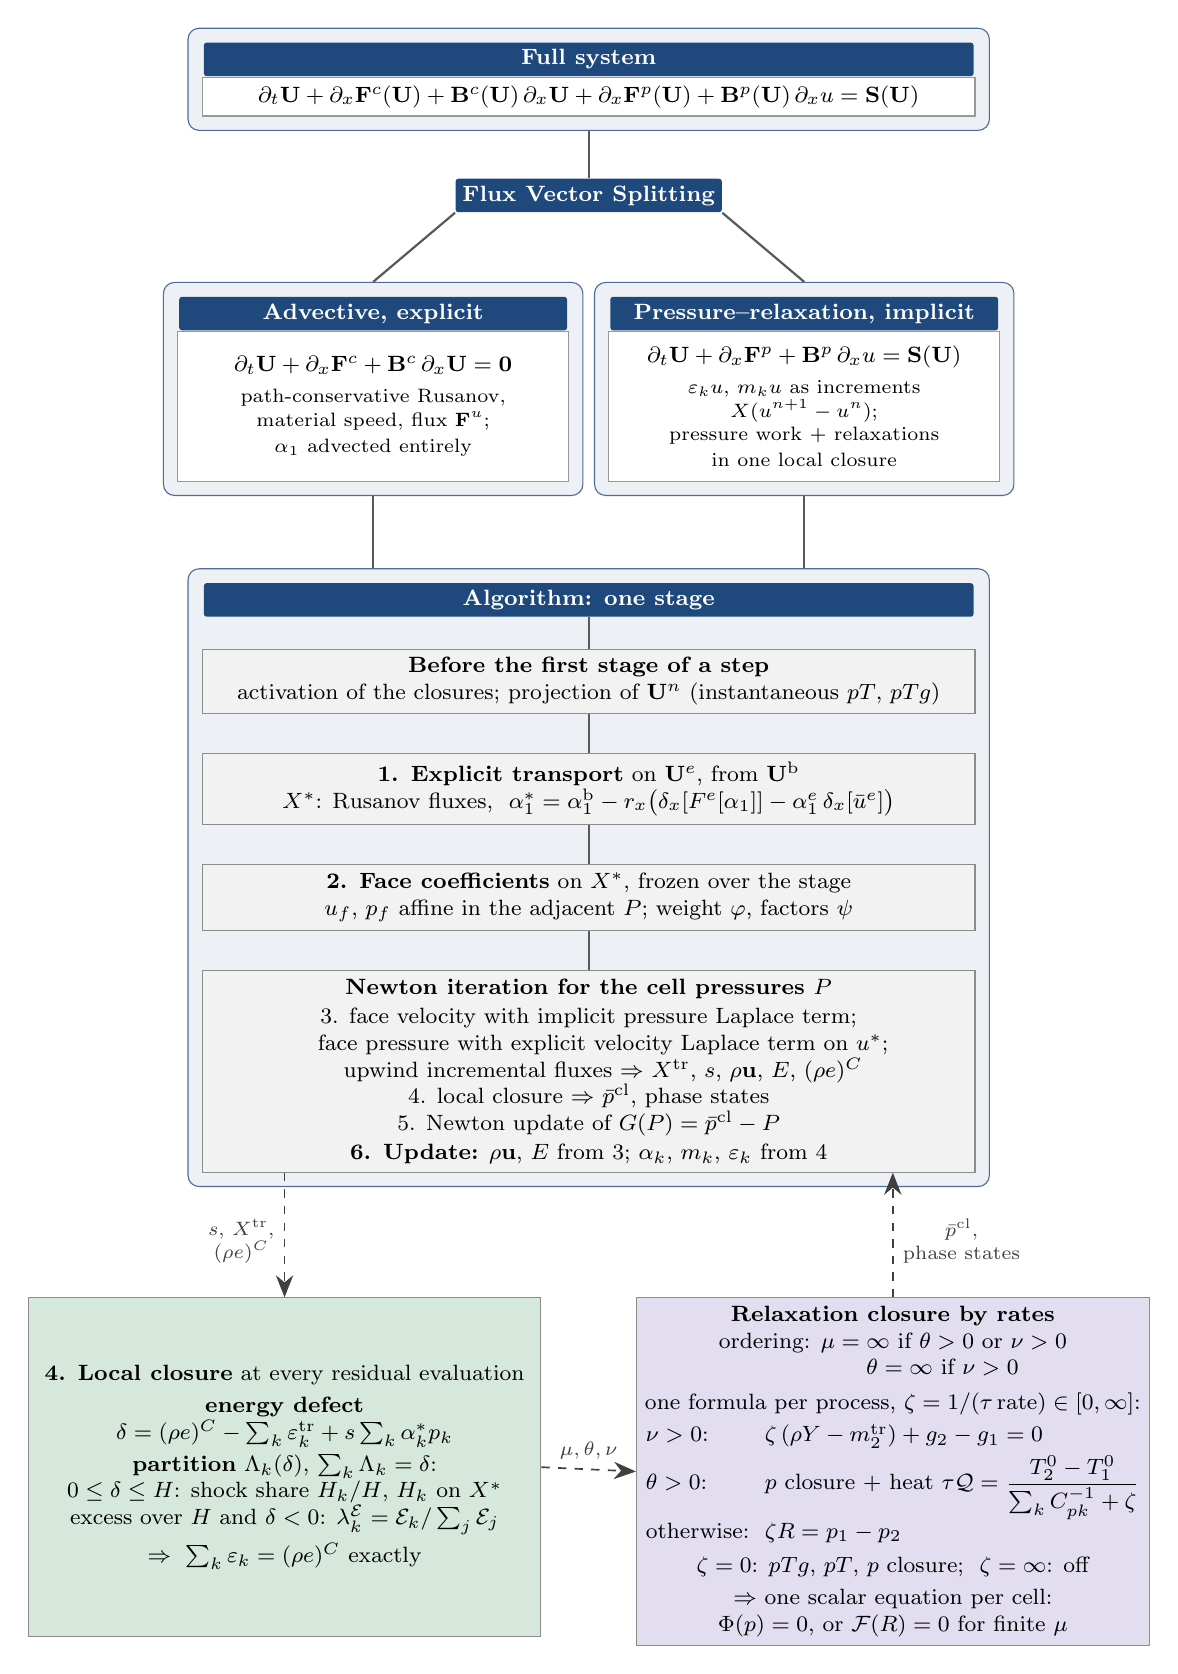
\begin{tikzpicture}[
  font=\fontsize{8pt}{9.6pt}\selectfont, >={Stealth[length=2.8mm,width=2.2mm]}, node distance=4mm,
  hdr/.style={fill=hdrblue, text=white, font=\fontsize{8pt}{9.6pt}\selectfont\bfseries, inner sep=2.5pt, rounded corners=1pt,
              align=flush center},
  eq/.style={draw=black!40, fill=white, inner sep=3pt, align=flush center},
  outer/.style={draw=hdrblue!80, fill=hdrblue!8, rounded corners=4pt, inner sep=5pt},
  step/.style={draw=black!45, fill=black!5, align=flush center, inner sep=3pt, text width=#1},
  step/.default=9.6cm,
  note/.style={align=flush center, font=\fontsize{7pt}{8.4pt}\selectfont},
  dashedarrow/.style={->, dashed, semithick, black!75},
]
\definecolor{hdrblue}{RGB}{31,73,125}
\definecolor{clgreen}{RGB}{214,232,220}
\definecolor{rlpurple}{RGB}{226,222,240}

% ----------------------------------------------------------------- full system
\node[eq, text width=9.6cm] (full) {$\partial_t\mathbf U+\partial_x\mathbf F^c(\mathbf U)+\mathbf B^c(\mathbf U)\,\partial_x\mathbf U
  +\partial_x\mathbf F^p(\mathbf U)+\mathbf B^p(\mathbf U)\,\partial_xu=\mathbf S(\mathbf U)$};
\node[hdr, above=0pt of full.north, text width=9.6cm] (fullh) {Full system};
\begin{scope}[on background layer]
  \node[outer, fit=(full)(fullh)] (fullbox) {};
\end{scope}

\node[hdr, below=6mm of fullbox] (split) {Flux Vector Splitting};
\draw[thick, black!65] (fullbox.south) -- (split.north);

% ----------------------------------------------------------------- the two sub-systems
\node[eq, below left=15mm and 2.5mm of split.south, anchor=north east, text width=4.75cm, minimum height=1.9cm] (adv)
  {$\partial_t\mathbf U+\partial_x\mathbf F^c+\mathbf B^c\,\partial_x\mathbf U=\mathbf 0$\\[3pt]
   {\fontsize{7pt}{8.4pt}\selectfont path-conservative Rusanov,\\ material speed, flux $\mathbf F^u$;\\ $\alpha_1$ advected entirely}};
\node[hdr, above=0pt of adv.north, text width=4.75cm] (advh) {Advective, explicit};
\node[eq, below right=15mm and 2.5mm of split.south, anchor=north west, text width=4.75cm, minimum height=1.9cm] (prs)
  {$\partial_t\mathbf U+\partial_x\mathbf F^p+\mathbf B^p\,\partial_xu=\mathbf S(\mathbf U)$\\[3pt]
   {\fontsize{7pt}{8.4pt}\selectfont $\varepsilon_ku$, $m_ku$ as increments $X(u^{n+1}-u^n)$;\\ pressure work $+$ relaxations\\ in one local closure}};
\node[hdr, above=0pt of prs.north, text width=4.75cm] (prsh) {Pressure--relaxation, implicit};
\begin{scope}[on background layer]
  \node[outer, fit=(adv)(advh)] (advbox) {};
  \node[outer, fit=(prs)(prsh)] (prsbox) {};
\end{scope}
\draw[thick, black!65] (split.south west) -- (advbox.north);
\draw[thick, black!65] (split.south east) -- (prsbox.north);

% ----------------------------------------------------------------- one stage (steps numbered as in Sec. 3.6)
\node[hdr, below=11mm of split.south |- advbox.south, text width=9.6cm] (alh) {Algorithm: one stage};
\node[step, below=4mm of alh] (s0)
  {\textbf{Before the first stage of a step}\\ activation of the closures; projection of $\mathbf U^n$ (instantaneous $pT$, $pTg$)};
\node[step, below=5mm of s0] (s1)
  {\textbf{1. Explicit transport} on $\mathbf U^e$, from $\mathbf U^{\rm b}$\\
   $X^*$: Rusanov fluxes, \ $\alpha^*_1=\alpha^{\rm b}_1-r_x\big(\delta_x[F^e[\alpha_1]]-\alpha^e_1\,\delta_x[\bar u^e]\big)$};
\node[step, below=5mm of s1] (s2)
  {\textbf{2. Face coefficients} on $X^*$, frozen over the stage\\ $u_f$, $p_f$ affine in the adjacent $P$; weight $\varphi$, factors $\psi$};
\node[step, below=5mm of s2] (s3)
  {\textbf{Newton iteration for the cell pressures $P$}\\[1pt]
   3. face velocity with implicit pressure Laplace term;\\
   \phantom{3. }face pressure with explicit velocity Laplace term on $u^*$;\\
   \phantom{3. }upwind incremental fluxes $\Rightarrow$ $X^{\rm tr}$, $s$, $\rho\mathbf u$, $E$, $(\rho e)^C$\\
   4. local closure $\Rightarrow$ $\bar p^{\rm cl}$, phase states\\
   5. Newton update of $G(P)=\bar p^{\rm cl}-P$\\[1pt]
   \textbf{6. Update:} $\rho\mathbf u$, $E$ from 3; $\alpha_k$, $m_k$, $\varepsilon_k$ from 4};
\begin{scope}[on background layer]
  \node[outer, fit=(alh)(s0)(s1)(s2)(s3)] (algbox) {};
\end{scope}
\draw[thick, black!65] (advbox.south) -- (advbox.south |- algbox.north);
\draw[thick, black!65] (prsbox.south) -- (prsbox.south |- algbox.north);
\draw[thick, black!65] (alh) -- (s0); \draw[thick, black!65] (s0) -- (s1); \draw[thick, black!65] (s1) -- (s2); \draw[thick, black!65] (s2) -- (s3);

% ----------------------------------------------------------------- local closure with energy partition
\node[step=6.3cm, fill=clgreen, draw=black!45, below left=14mm and 6mm of algbox.south, anchor=north east, minimum height=4.3cm] (cl)
  {\textbf{4. Local closure} at every residual evaluation\\[2pt]
   \textbf{energy defect}\\ $\delta=(\rho e)^C-\sum_k\varepsilon^{\rm tr}_k+s\sum_k\alpha^*_kp_k$\\[2pt]
   \textbf{partition} $\Lambda_k(\delta)$, $\sum_k\Lambda_k=\delta$:\\
   $0\le\delta\le H$: shock share $H_k/H$, $H_k$ on $X^*$\\
   excess over $H$ and $\delta<0$: $\lambda^{\mathcal E}_k=\mathcal E_k/\sum_j\mathcal E_j$\\[2pt]
   $\Rightarrow\ \sum_k\varepsilon_k=(\rho e)^C$ exactly};

% ----------------------------------------------------------------- relaxation closures by rates
\node[step=6.3cm, fill=rlpurple, draw=black!45, below right=14mm and 6mm of algbox.south, anchor=north west, minimum height=4.3cm] (rl)
  {\textbf{Relaxation closure by rates}\\
   ordering: $\mu=\infty$ if $\theta>0$ or $\nu>0$\\ \phantom{ordering:} $\theta=\infty$ if $\nu>0$\\[3pt]
   one formula per process, $\zeta=1/(\tau\,{\rm rate})\in[0,\infty]$:\\[2pt]
   \begin{tabular}{@{}l@{\ \ }l@{}}
   $\nu>0$:      & $\zeta\,(\rho Y-m^{\rm tr}_2)+g_2-g_1=0$\\[2pt]
   $\theta>0$:   & $p$ closure $+$ heat $\tau\mathcal Q=\dfrac{T^0_2-T^0_1}{\sum_kC_{pk}^{-1}+\zeta}$\\[6pt]
   otherwise:    & $\zeta R=p_1-p_2$
   \end{tabular}\\[3pt]
   $\zeta=0$: $pTg$, $pT$, $p$ closure;\ \ $\zeta=\infty$: off\\[2pt]
   $\Rightarrow$ one scalar equation per cell:\\ $\Phi(p)=0$, or $\mathcal F(R)=0$ for finite $\mu$};

\draw[dashedarrow] (s3.south -| cl.north) -- node[pos=0.55, left, note] {$s$, $X^{\rm tr}$,\\$(\rho e)^C$} (cl.north);
\draw[dashedarrow] (cl.east) -- node[above, note] {$\mu,\theta,\nu$} (rl.west);
\draw[dashedarrow] (rl.north) -- node[pos=0.45, right, note] {$\bar p^{\rm cl}$,\\phase states} (s3.south -| rl.north);

\end{tikzpicture}
}
\caption{Schematic of the semi-implicit scheme. The Toro--V\'azquez-Cend\'on splitting separates the advective
sub-system, advanced explicitly with the old-velocity part of the internal energy fluxes, from the pressure--relaxation
sub-system, solved implicitly with the increments of the mass and internal energy fluxes. Every residual evaluation of the pressure system calls the local closure of each cell, which
distributes the energy defect $\delta$ between the phases, and the relaxation closure selected by the rates.}
\label{fig:scheme}
\end{figure}
\clearpage



\subsection{Fully discrete scheme in two dimensions}
\label{sec:fully}
One stage of the scheme, with the explicit state $\mathbf U^e=\mathbf U_{E,i}$, the update base $\mathbf U^{\rm b}=\tilde{\mathbf U}_{I,i}$ and the implicit step
$\tau=a_{ii}\Delta t$, or $\mathbf U^e=\mathbf U^{\rm b}=\mathbf U^n$ and $\tau=\Delta t$ in a first-order step, consists of the following steps, with $r_x=\tau/\Delta x$
and $r_y=\tau/\Delta y$. Before the first stage of a step the closures are activated and $\mathbf U^n$ is projected as in
Sec.~\ref{sec:relaxation}.
\begin{enumerate}
\item \emph{Explicit transport.} The face values are reconstructed on $\mathbf U^e$ by \eqref{eq:shared_limiter} with the cap \eqref{eq:phi_cap}, and every
transported quantity is advanced with the Rusanov fluxes \eqref{eq:rusanov},
\[
X^*_{i,j}=X^{\rm b}_{i,j}-r_x\,\delta_x\big[F^e[X]\big]_{i,j}-r_y\,\delta_y\big[G^e[X]\big]_{i,j},\quad
X\in\{m_k,\varepsilon_k,\rho u,\rho v,E\},
\]
and the volume fraction by the path-conservative update
\eqref{eq:alpha_explicit} with base $\alpha^{\rm b}_1$ and the cell's own volume fraction $\alpha^e_1$ of $\mathbf U^e$ in the strain term,
\[
\begin{aligned}
\alpha^*_{1,i,j}=\alpha^{\rm b}_{1,i,j}&-r_x\Big(\delta_x\big[F^e[\alpha_1]\big]_{i,j}-\alpha^e_{1,i,j}\,\delta_x[\bar u^e]_{i,j}\Big)\\
&-r_y\Big(\delta_y\big[G^e[\alpha_1]\big]_{i,j}-\alpha^e_{1,i,j}\,\delta_y[\bar v^e]_{i,j}\Big),\qquad \alpha^*_2=1-\alpha^*_1 .
\end{aligned}
\]
\item \emph{Face coefficients.} On every face the quantities of Sec.~\ref{sec:dissipation} are computed from $X^*$, the
limiter factors of the reconstruction of $\mathbf U^e$ and the pressures of the previous stage: the averages $\bar u^*_f$, $\bar\rho_f$, the impedances $Z$, the weight \eqref{eq:weight},
the factors \eqref{eq:psi} and the velocity jump \eqref{eq:vertex_div}. They are frozen during the solution of the stage,
so that the face velocity and face pressure \eqref{eq:faces} are affine in the two adjacent cell pressures,
\[
u_f=\bar u^*_f-\Theta_f\,(P_R-P_L),\qquad p_f=W_fP_L+(1-W_f)P_R-\varpi_f ,
\]
with $\Theta_f=\tau/(\bar\rho_f h)+\eta^P_f/h$, $W_f=\rho^*_R/(\rho^*_L+\rho^*_R)$ and $\varpi_f=\eta^u_fD^*_f/h$, $h=\Delta x$ or $\Delta y$. At a non-periodic boundary the
ghost cells take the pressure of the adjacent cell, or the given pressure at the outlet of Sec.~\ref{sec:res_bartak}, and their state is a copy of the boundary cells at transmissive
boundaries and their mirror image at walls, with the normal velocity $2u_w-u$ for a wall velocity $u_w$; on a wall face $u_f=u_w$. At periodic boundaries the ghost cells and their pressures are those of the opposite side.
\item \emph{Incremental fluxes and conservative updates.} For given cell pressures, the incremental fluxes
\eqref{eq:increment} are split into their donor parts $I_f=I^L_f+I^R_f$; the incremental mass fluxes are
$\hat M^{L,R}_f=\sum_kI^{L,R}_f[m_k]$, $\hat M_f=\hat M^L_f+\hat M^R_f$. Then
\[
\begin{aligned}
&X^{\rm tr}_{i,j}=X^*_{i,j}-r_x\,\delta_x\big[I[X]\big]_{i,j}-r_y\,\delta_y\big[I[X]\big]_{i,j},\qquad X\in\{m_k,\varepsilon_k\},\\
&s_{i,j}=r_x\,\delta_x[u_f]_{i,j}+r_y\,\delta_y[v_f]_{i,j},\qquad \alpha^{\rm tr}_{k,i,j}=\alpha^*_{k,i,j}(1-s_{i,j}),\\
&\rho^{\rm new}_{i,j}=\textstyle\sum_km^{\rm tr}_{k,i,j}.
\end{aligned}
\]
Let $u_\perp$ be the normal face velocity, $u_f$ on $x$-faces and $v_f$ on $y$-faces, and $u_{\parallel,L}$, $u_{\parallel,R}$ the tangential velocities
of $X^*$ in the two cells of the face, $v^*$ on $x$-faces and $u^*$ on $y$-faces. The momentum is advanced with the face
pressure and the incremental momentum flux, normal and tangential,
\[
\begin{aligned}
(\rho u)^{\rm new}_{i,j}&=(\rho u)^*_{i,j}-r_x\,\delta_x\big[p_f+u_\perp\hat M_f\big]_{i,j}-r_y\,\delta_y\big[u_{\parallel,L}\hat M^L_f+u_{\parallel,R}\hat M^R_f\big]_{i,j},\\
(\rho v)^{\rm new}_{i,j}&=(\rho v)^*_{i,j}-r_x\,\delta_x\big[u_{\parallel,L}\hat M^L_f+u_{\parallel,R}\hat M^R_f\big]_{i,j}-r_y\,\delta_y\big[p_f+u_\perp\hat M_f\big]_{i,j},
\end{aligned}
\]
and the total energy with the energy flux
\[
\begin{gathered}
F^I_f[E]=\textstyle\sum_kI_f[\varepsilon_k]+\tfrac12u_\perp^2\hat M_f+\tfrac12\big(u_{\parallel,L}^2\hat M^L_f+u_{\parallel,R}^2\hat M^R_f\big)+p_fu_\perp ,\\
E^{\rm new}_{i,j}=E^*_{i,j}-r_x\,\delta_x\big[F^I[E]\big]_{i,j}-r_y\,\delta_y\big[F^I[E]\big]_{i,j}.
\end{gathered}
\]
In each cell the conservative mixture internal energy is $(\rho e)^C=E^{\rm new}-|(\rho\mathbf u)^{\rm new}|^2/(2\rho^{\rm new})$.
\item \emph{Local closure.} In every cell the defect \eqref{eq:defect} is partitioned by \eqref{eq:Lambda}, with the
physical budget \eqref{eq:Qk} computed on $X^*$ after step 1 and frozen during the stage, and the relaxation closure of
Sec.~\ref{sec:relaxation} returns $\bar p^{\rm cl}_{i,j}$ and the phase states.
\item \emph{Pressure system.} The system \eqref{eq:global} is solved for the cell pressures by the Newton method of
Sec.~\ref{sec:pressure_system}; every residual evaluation repeats steps 3 and 4.
\item \emph{Update.} At the converged pressures, the stage value consists of the momentum and the total energy of
step 3 and the volume fractions, partial densities and phase energies of the closure of step 4.
\end{enumerate}
Steps 1--6 give the stage value $\mathbf U_i$ of \eqref{eq:stages}, step 1 being its explicit part and steps 2--6 its implicit part.






% =====================================================================
% Section 4. Numerical results  (structure as Battisti & Boscheri 2025 and Chen et al. 2026, Sec. 4)
% Source: src/spb6_physics.h (test_setup, test_state), tests/run_archive.sh, data/*/note.md
% Only the test descriptions and initial data are written; the results are to be added.
% =====================================================================
\section{Numerical results}
\label{sec:results}

In this section we validate the proposed semi-implicit scheme on a suite of test problems, following the order in
which the ingredients of the method are introduced. We begin by assessing the accuracy of the full scheme on a smooth
two-phase vortex, measuring the experimental order of convergence as the Mach number is decreased. We then turn to
one-dimensional problems: the advection of material interfaces, which checks the well-balanced property; single-phase
Riemann problems over a wide range of Mach numbers; shock tubes with mechanical relaxation, with stiffened-gas and
Mie--Gr\"uneisen equations of state and with a shock in a two-phase mixture, which checks the distribution of the
energy defect; and expansion, evaporation and depressurisation problems with thermal and chemical relaxation, at
instantaneous and finite rates. The low Mach number limit of the mixture is then examined on the Taylor--Green
vortex. Finally, we consider two-dimensional problems with interfaces, shocks, cavitation and phase transition.

Unless otherwise stated, all computations use the scheme of Sec.~\ref{sec:method} with LSDIRK2, the material CFL condition
\eqref{eq:cfl} with $C=0.2$, minmod reconstruction, a local Rusanov speed on each face and the Newton tolerance of
Sec.~\ref{sec:pressure_system} and the start-up rule of Sec.~\ref{sec:time}. Thermal and chemical relaxation
are active in cells with $10^{-4}\le\alpha_1\le1-10^{-4}$. Where a phase is absent its volume fraction is set to $10^{-8}$, $10^{-7}$ or
$10^{-6}$ as indicated; initial data in two dimensions are cell averages computed with $4\times4$ sub-cells. Units are SI
unless stated otherwise.

Mechanical relaxation is instantaneous in all tests; finite rates are used for thermal and chemical relaxation only.
The relaxation levels are denoted as in Pelanti and Shyue \cite{PelantiShyue2014}. $p$: instantaneous mechanical relaxation only.
$p$--$pT$: in addition, instantaneous thermal relaxation in interface cells. $p$--$pT$--$pTg$: in addition, instantaneous
mass transfer in interface cells where the $pT$-equilibrium temperature exceeds $T_{\rm sat}(p)$. A finite rate replaces the
corresponding instantaneous relaxation and is marked $(f)$. Reference solutions are exact Riemann solutions of the
relaxed limit models: the five-equation model for $p$, the four-equation model for $p$--$pT$, and the $pT\to pTg$ wave
fan and the homogeneous equilibrium model for instantaneous mass transfer.

% ---------------------------------------------------------------------
\subsection{Accuracy of the numerical scheme: two-phase isentropic vortex}
\label{sec:res_vortex}
This test of Battisti and Boscheri \cite[Sec.~4.1]{BattistiBoscheri2025} measures the order of accuracy for a smooth two-phase flow at decreasing
Mach number. The domain is $[-5,5]^2$ with periodic boundaries; phase 1 is an ideal gas with $\gamma_1=1.35$ and
phase 2 an ideal gas with $\gamma_2=1.4$. With $r^2=x^2+y^2$, $\varepsilon=5$ and $\gamma=1.4$,
\begin{equation}
\begin{aligned}
&u=2-\frac{\varepsilon}{2\pi}e^{(1-r^2)/2}\,y,\qquad v=2+\frac{\varepsilon}{2\pi}e^{(1-r^2)/2}\,x,\qquad
T=p_0-\frac{(\gamma-1)\varepsilon^2}{8\gamma\pi^2}e^{1-r^2},\\
&\rho_1=\rho_2=\Big(\frac{T}{p_0}\Big)^{1/(\gamma-1)},\qquad p_1=p_2=\rho_1T,\qquad \alpha_2=\frac12+\frac14e^{(1-r^2)/2}.
\end{aligned}
\label{eq:vortex}
\end{equation}
The phases have equal pressure and density, the velocity field is divergence-free and $\alpha_2$ and the entropy are
constant along streamlines, so the exact solution is the translation of \eqref{eq:vortex} with velocity $(2,2)$; at
$t=5$ it coincides with the initial data. The background pressure is $p_0=1,10,10^2,10^3,10^4$, which gives
$M=2\sqrt2/\sqrt{\gamma p_0}$ from $2.4$ to $0.024$, and the grids have $N^2$ cells with $N=32,64,128,256$. Two initial
data are used. In the first the cell averages of \eqref{eq:vortex} are taken. In the second, well-prepared, the
velocity is the central difference of the stream function $\psi=\frac{\varepsilon}{2\pi}e^{(1-r^2)/2}$ at the cell
centres, $u_{i,j}=2+(\psi_{i,j+1}-\psi_{i,j-1})/(2\Delta y)$, $v_{i,j}=2-(\psi_{i+1,j}-\psi_{i-1,j})/(2\Delta x)$, which is discretely
divergence-free; the other variables are cell
averages. In both cases the errors are measured in $L_2$ against the $4\times4$-point cell averages of the exact solution. The slopes are the unlimited central differences.

% ---------------------------------------------------------------------
\subsection{One-dimensional Riemann problems}
\label{sec:res_1d}
The following problems in one space dimension test the scheme on material interfaces, on single-fluid waves over a wide
range of Mach numbers and on shocks with mechanical relaxation.

% ---------------------------------------------------------------------
\subsubsection{Interface advection}
\label{sec:res_interface}
A water--air interface is advected in $[0,1]$ with transmissive boundaries \cite[Sec.~4.1]{SPB2009}. Water is a
stiffened gas with $\gamma=4.4$, $\pi=6\times10^8$\,Pa, air an ideal gas with $\gamma=1.4$. Initially $u=100$\,m/s,
$p=10^5$\,Pa, $\rho_{\rm water}=1000$, $\rho_{\rm air}=10$, and $\alpha_{\rm water}=1-10^{-8}$ for $x<0.5$, $10^{-8}$ otherwise. The
computation uses 200 cells and ends at $t=2.79$\,ms, when the interface is at $x=0.779$. Two low-Mach variants follow
Schropff et al.\ \cite{Schropff2026}: the same fluids with $u=1$\,m/s, $\rho_{\rm air}=0.01$, $\alpha_{\rm water}=1-10^{-7}$ for $x<0.25$ and $10^{-7}$
otherwise, $t_{\rm end}=0.25$\,s, so that $M=|u|/c$ lies between $2.7\times10^{-4}$ in the air and $6\times10^{-4}$ in the water; and a single gas, air, with a density step $\rho=1000$ for $x<0.25$
and $\rho=0.01$ otherwise, $u=1$\,m/s, $p=10^5$\,Pa, $t_{\rm end}=0.5$\,s, so that $M$ ranges from $2.7\times10^{-4}$ to
$8.5\times10^{-2}$. Both use 200 and 1000 cells. In all three cases uniform velocity and pressure must be preserved
(Proposition~\ref{prop:wb}).

% ---------------------------------------------------------------------
\subsubsection{Single-phase Riemann problems}
\label{sec:res_single}
The Riemann problems of Table~\ref{tab:single} \cite[Secs.~5.1, 5.1.1]{Schropff2026} test the scheme for a single fluid over a wide
range of Mach numbers. A single fluid is represented by two identical phases in the same state, with
$\alpha_1=1-10^{-8}$. Air is an ideal gas with $\gamma=1.4$ and water the stiffened gas of Sec.~\ref{sec:res_interface}. The
domain is $[0,1]$ with transmissive boundaries, the initial discontinuity is at $x=0.5$, and 200 and 1000 cells are
used. The reference is the exact solution of the Euler equations.
\begin{table}[t]
\centering\small
\caption{Single-phase Riemann problems \cite{Schropff2026}: left and right states and final time.}
\label{tab:single}
\begin{tabular}{lllll}
\toprule
problem & fluid & $(\rho,u,p)_L$ & $(\rho,u,p)_R$ & $t_{\rm end}$ \\
\midrule
low-Mach shock tube & water & $(1000,\ 0,\ 10^8)$ & $(1000,\ 15,\ 0.98\times10^8)$ & $10^{-4}$ \\
liquid--liquid shock tube & water & $(1000,\ 0,\ 10^6)$ & $(1000,\ 0,\ 10^5)$ & $1.5\times10^{-4}$ \\
Lax shock tube & air & $(0.445,\ 0.698,\ 3.528)$ & $(0.5,\ 0,\ 0.571)$ & 0.14 \\
strong shock tube & air & $(1,\ 0,\ 10^{10})$ & $(0.125,\ 0,\ 0.1)$ & $2.5\times10^{-6}$ \\
two rarefactions & air & $(1,\ -1,\ 0.4)$ & $(1,\ 1,\ 0.4)$ & 0.15 \\
\bottomrule
\end{tabular}
\end{table}

% ---------------------------------------------------------------------
\subsubsection{Shock tubes with mechanical relaxation}
\label{sec:res_shock}
The following Riemann problems on $[0,1]$, or $[-10,10]$ for the detonation products, with transmissive boundaries
are computed with the $p$ relaxation and compared with the exact solution of the five-equation model. The fluids are
at rest initially.

\paragraph{Water--air shock tube}
Water and air as in Sec.~\ref{sec:res_interface} \cite[Sec.~4.3.1]{SPB2009}. For $x<0.75$, water with
$\alpha_{\rm water}=1-10^{-6}$, $\rho=1000$, $p=10^9$\,Pa; for $x>0.75$, air with $\alpha_{\rm air}=1-10^{-6}$, $\rho=1$, $p=10^5$\,Pa;
$t_{\rm end}=240\,\mu$s, with 1000 and 100 cells.

\paragraph{Nitromethane shock tube}
Both phases are liquid nitromethane with the Cochran--Chan law \eqref{eq:mg_ref} \cite[Sec.~4.2]{SPB2009}
with $\Gamma=1.19$, $\rho_0=1134$, $A_1=0.819181$\,GPa, $A_2=1.50835$\,GPa, $E_1=4.52969$, $E_2=1.42144$. Phase 1 has
$\rho_1=1134$ and phase 2 $\rho_2=1200$; $\alpha_1=1-10^{-8}$, $p=2\times10^{10}$\,Pa for $x<0.5$ and $\alpha_1=10^{-8}$,
$p=2\times10^5$\,Pa otherwise. 500 cells, $t_{\rm end}=67\,\mu$s. The nonlinear reference curve makes the contact
discontinuity a test of pressure and velocity oscillations.

\paragraph{Detonation products--water shock tube}
Detonation products follow the JWL law \eqref{eq:mg_ref} \cite[Sec.~8.1.1]{Pelanti2022}
with $\Gamma=0.25$, $\rho_0=1840$, $A=854.5$\,GPa, $B=20.5$\,GPa, $R_1=4.6$, $R_2=1.35$; water is NASG with $(\gamma,\pi,q,q',c_v,b)=
(1.187,\ 7.028\times10^8,\ -1177788,\ 0,\ 3610,\ 6.61\times10^{-4})$. On $[-10,10]$, the products ($\alpha=1-10^{-8}$, $\rho=2000$,
$p=4.6406\times10^{10}$\,Pa) fill $x<0$ and water ($\rho=1044$, $p=10^5$\,Pa) $x>0$. 500 cells, $t_{\rm end}=0.9$\,ms.

\paragraph{Epoxy--spinel mixture}
A mixture of epoxy (SG, $\gamma=2.43$, $\pi=5.3\times10^9$\,Pa) and spinel (SG, $\gamma=1.62$, $\pi=1.41\times10^{11}$\,Pa) with
$\alpha_{\rm epoxy}=0.5954$, $\rho_{\rm epoxy}=1185$, $\rho_{\rm spinel}=3622$ everywhere \cite[Sec.~5.2]{SPB2009}. The pressure
is $2\times10^{11}$\,Pa for $x<0.6$ and $10^5$\,Pa otherwise; 500 cells, $t_{\rm end}=34\,\mu$s, global Rusanov speed. Both phases
are compressed through the same shock; the test checks the partition of the energy defect of Sec.~\ref{sec:closure}.

% ---------------------------------------------------------------------
\subsection{Water cavitation tube}
\label{sec:res_cav}
Two streams of liquid water moving apart from $x=0.5$ in $[0,1]$, with transmissive boundaries, produce a strong
expansion at the centre \cite[Sec.~8.2.1]{Pelanti2022}. Water is NASG with liquid $(1.187,\ 7.028\times10^8,\ -1177788,\ 0,\ 3610,\ 6.61\times10^{-4})$
and vapour $(1.467,\ 0,\ 2077616,\ 14317,\ 955,\ 0)$. Initially $\alpha_v=10^{-2}$, both phases at $p=10^5$\,Pa and $T_0=353$\,K with
$\rho_k=\rho_k(p,T_0)$, and $u=-2$\,m/s for $x<0.5$, $+2$\,m/s otherwise; 5000 cells, $t_{\rm end}=3$\,ms. The same configuration
is computed with five levels: $p$; $p$--$pT(f)$ with $\theta=2000$; $p$--$pT$; $p$--$pT$--$pTg(f)$ with $\nu=10^{-4}$; $p$--$pT$--$pTg$.

% ---------------------------------------------------------------------
\subsection{Dodecane liquid--vapour shock tube}
\label{sec:res_dodecane}
Liquid dodecane at high pressure expands into its vapour \cite[Sec.~8.2.2]{Pelanti2022}.
Dodecane is NASG with liquid $(1.206,\allowbreak\ 1.681\times10^8,\allowbreak\ -996054,\allowbreak\ 0,\allowbreak\ 2532,\allowbreak\ 7.51\times10^{-4})$ and vapour
$(1.021,\ 0,\ -384592,\ -4301,\ 2274,\ 0)$. For $x<0.75$, liquid with $\alpha_l=1-10^{-8}$, $\rho_l=500$, $p=10^8$\,Pa; for $x>0.75$,
vapour with $\alpha_v=1-10^{-8}$, $\rho_v=2$, $p=10^5$\,Pa; transmissive boundaries, 2000 cells, $t_{\rm end}=473\,\mu$s; levels $p$
and $p$--$pT$--$pTg$.

% ---------------------------------------------------------------------
\subsection{Bart\'ak rapid depressurisation}
\label{sec:res_bartak}
A pipe of length 1.7\,m filled with hot pressurised water is opened at one end \cite[Sec.~8.2.4]{Pelanti2022}, after the experiment of Bart\'ak \cite{Bartak1990}. Water is
NASG with liquid $(1.387,\ 8.899\times10^8,\ -1244191,\ 0,\ 3202,\ 4.78\times10^{-4})$ and vapour $(1.954,\ 0,\ 2287484,\ 6417,\ 462,\ 0)$.
Initially $p=12.5$\,MPa, $T=563.15$\,K, $u=0$, $\alpha_v=10^{-3}$ and $\rho_k=\rho_k(p,T)$. The right end $x=1.7$ is a wall; at the
left end the pressure $10^5$\,Pa is imposed: the ghost cells keep $\alpha$, $m_k$ and $u$ of the adjacent cell with both
phase pressures equal to $10^5$\,Pa, and this pressure is a given value in the pressure system. 1000 cells,
$t_{\rm end}=17.5$\,ms; pressure and vapour mass fraction are recorded at $x=48$\,mm. Three cases are computed with
instantaneous thermal relaxation: no mass transfer ($p$--$pT$), instantaneous mass transfer ($p$--$pT$--$pTg$), and the
finite rate
\begin{equation}
\nu=C_r\,\alpha_v^{0.6}\Big(\frac{p_{\rm sat}(T)-p}{p_{\rm crit}-p_{\rm sat}(T)}\Big)^{1.76}\quad(p<p_{\rm sat}(T)),\qquad \nu=0\ \text{otherwise},
\label{eq:bartak_nu}
\end{equation}
with $C_r=1$ and $p_{\rm crit}=22.064$\,MPa, evaluated in each cell from its $pT$-equilibrium state at the beginning of the
step and frozen over the stages. With instantaneous mass transfer the solution at the probe is a simple wave of the
homogeneous equilibrium model, which is computed exactly.

% ---------------------------------------------------------------------
\subsection{Low Mach number limit: Taylor--Green vortex}
\label{sec:res_tg}
This test of Battisti and Boscheri \cite[Sec.~4.4]{BattistiBoscheri2025} checks the low-Mach limit of Sec.~\ref{sec:ap}. On $[0,2\pi]^2$ with periodic
boundaries both phases are ideal gases with $\gamma=1.4$, and
\begin{equation}
\rho_1=\rho_2=1,\qquad u=\sin x\cos y,\qquad v=-\cos x\sin y,\qquad p_1=p_2=p_0+\tfrac14(\cos2x+\cos2y),
\label{eq:tg}
\end{equation}
a stationary solution of the incompressible Euler equations \cite{TaylorGreen1937}. The volume fraction is $\alpha_2=\tfrac12$ in the single-phase
case and $\alpha_2=\tfrac12+\tfrac1{10}(\cos2x+\cos2y)$ in the two-phase case. The background pressure
$p_0=10^2,10^4,\dots,10^{12}$ gives $M=1/\sqrt{1.4\,p_0}$ from $8.45\times10^{-2}$ to $8.45\times10^{-7}$. On a $50\times50$ grid the
solution is computed to $t=0.2$ with the fixed time step $\Delta t=2.5\times10^{-3}$, independent of $M$; the order of
accuracy is measured for $p_0=10^6$ and $10^{10}$ on $N=32,\dots,256$ with $\Delta t=0.08/N$. Both computations are made with
unlimited central slopes and with minmod. The errors are measured in $L_2$ against the $4\times4$-point cell averages of
\eqref{eq:tg}, together with the discrete divergence of the face velocities.
% ---------------------------------------------------------------------
\subsection{Shock--helium bubble interaction}
\label{sec:res_he}
A Mach 1.5 shock in air hits a helium bubble \cite[Sec.~4.6]{SPB2009}, after the experiment of Layes and Le M\'etayer \cite{LayesLeMetayer2007}. The domain is $[0,0.3]\times[0,0.08]$ with
walls at $y=0$ and $y=0.08$ and transmissive boundaries in $x$; air is an ideal gas with $\gamma=1.4$, helium with
$\gamma=1.67$. The bubble has diameter 0.04 and centre $(0.2,0.04)$; inside $\alpha_{\rm air}=10^{-6}$, outside $1-10^{-6}$. Ahead
of the shock, air has $\rho=1.29$, $p=101325$\,Pa and helium $\rho=0.167$, both at rest. The shock is at $x=0.221$ and
moves to the left; behind it the air state follows from the Rankine--Hugoniot relations of the ideal gas at Mach 1.5.
$600\times160$ cells, $t_{\rm end}=600\,\mu$s, $p$ relaxation.

% ---------------------------------------------------------------------
\subsection{Cavitating Richtmyer--Meshkov instability}
\label{sec:res_rm}
A water column with a curved surface moving at $-200$\,m/s hits a wall \cite[Sec.~4.7]{SPB2009}. On $[0,3]\times[0,1]$,
water (SG, $\gamma=4.4$, $\pi=6\times10^8$\,Pa, $\rho=1000$) occupies $x<1.2+\sqrt{0.36-(y-0.5)^2}$ and gas (ideal, $\gamma=1.8$,
$\rho=100$) the rest, with $\alpha=1-10^{-6}$ for the present phase; everywhere $u=-200$\,m/s and $p=101325$\,Pa. The left,
bottom and top boundaries are walls and the right boundary is transmissive. $300\times100$ cells, the grid of Pelanti and Shyue \cite[Sec.~5.3]{PelantiShyue2014}, $t_{\rm end}=8.6$\,ms,
$p$ relaxation, global Rusanov speed.

% ---------------------------------------------------------------------
\subsection{Compression of a vapour bubble}
\label{sec:res_bubble}
A dodecane vapour bubble in liquid dodecane is compressed by a piston \cite[Sec.~5.4]{PelantiShyue2014}. Dodecane is SG
with liquid $(2.35,\ 4\times10^8,\ -775.269\times10^3,\ 0,\ 1077.7)$ and vapour $(1.025,\ 0,\ -237.547\times10^3,\ -24.4\times10^3,\ 1956.45)$. On $[0,1]^2$ a bubble of radius 0.2 is centred at $(0.5,0.5)$;
initially $p=10^5$\,Pa and $T=600$\,K, so $\rho_l=458.338$ and $\rho_v=3.408$, with $\alpha_l=10^{-6}$ inside the bubble and
$\alpha_v=10^{-6}$ outside, at rest. All boundaries are walls; the left wall moves with velocity $100$\,m/s in $+x$; the grid
is fixed and the wall boundary condition imposes this normal velocity. $200\times200$ cells, $t_{\rm end}=1.2$\,ms,
$p$--$pT$--$pTg$ relaxation, global Rusanov speed.

% ---------------------------------------------------------------------
\subsection{Underwater explosion near a wall}
\label{sec:res_undex}
A bubble of detonation products expands in water below a rigid wall \cite[Sec.~8.1.2]{Pelanti2022}. The states and the
equations of state are those of the detonation products--water shock tube of Sec.~\ref{sec:res_shock}: products with
$\rho=2000$, $p=4.6406\times10^{10}$\,Pa and $\alpha=1-10^{-6}$ inside a circle of radius 0.05 centred at $(0,-0.32)$, water with
$\rho=1044$, $p=10^5$\,Pa outside. The domain is $[-1.35,1.35]\times[-1.5,0]$ with a wall at $y=0$ and transmissive
boundaries elsewhere. $361\times200$ cells, half the resolution of \cite{Pelanti2022}, $t_{\rm end}=0.4$\,ms, $p$ relaxation; the pressure is recorded at the wall
centre $(0,0)$.

% =====================================================================
% Section 5. Conclusions
% =====================================================================
\section{Conclusions}
\label{sec:conclusions}

We have presented a second-order semi-implicit IMEX finite volume scheme for the single-velocity six-equation
two-phase model with total energy, for stiffened-gas and Noble--Abel stiffened-gas phases with mechanical, thermal and
chemical relaxation and for Mie--Gr\"uneisen phases with instantaneous mechanical relaxation, in one and two space dimensions.

The two stiffnesses of the model, the acoustic waves at low Mach numbers and the relaxation processes up to infinite
rates, are treated in a single implicit step. The implicit pressure work and the three relaxation processes, each at a
finite or infinite rate, a slower process being active only when the faster ones are instantaneous \cite{Pelanti2022}, enter one local closure per cell, which reduces to a scalar equation in the
cell pressure or, for finite mechanical relaxation, in the volume increment; each stage then reduces to a nonlinear system
for the cell pressures with a three-point Jacobian, five-point in 2D, solved by Newton's method. The time step is restricted by the flow velocity only, whatever
the Mach number and the relaxation rates. We have proved that, at fixed mesh and under non-degeneracy assumptions, the scheme converges, for data on the
equilibrium manifold, to the corresponding equilibrium scheme as each relaxation rate tends to infinity and reduces to the scheme without that
relaxation as the rate vanishes; formally, it is asymptotic preserving in the low Mach number limit of the mixture.

At shocks, the difference between the conservative and the non-conservative mixture internal energy is distributed
between the phases according to the shock relations of the model: the physical part with the constant share for which
the shock profile of the relaxed model ends on the Hugoniot of each phase, computed by shooting, which for weak shocks
reduces to the unique consistent local share, and the discretisation error with the unique linear share that keeps both phases
admissible whenever possible. No calibrated heat exchange is needed.

The flux is split following Toro and V\'azquez-Cend\'on, with the mass and internal energy fluxes evaluated at the new
velocity: all quantities are transported explicitly with the old velocity by the path-conservative Rusanov scheme, whose
dissipation speed is the material speed, the volume fraction being advected entirely in this step, while the pressure,
its work on each phase and the increments of the mass and internal energy fluxes from the old to the new velocity are
treated implicitly. The central implicit operator is supplemented by Laplace dissipation of the
pressure and the velocity with acoustic coefficients, weighted by the deficit of the backward-Euler viscosity with respect to
the upwind one, so that it vanishes in the low Mach number regime; it is first order at local extrema and second order in
smooth regions. Second
order in time is obtained with the stiffly accurate, L-stable LSDIRK2 scheme. We have also proved that the scheme
preserves moving contacts between stiffened-gas or Noble--Abel stiffened-gas phases, at uniform temperature when thermal or
chemical relaxation is active.

The numerical results confirm these properties: second-order convergence of the velocity and the volume fraction on a
smooth two-phase vortex at Mach numbers from $2.4$ to $0.024$, and of the pressure for well-prepared data, face velocities
that are discretely divergence-free to $O(M^2)$ down to $M\approx10^{-6}$ on the Taylor--Green vortex with a time step
independent of the Mach number, and agreement with exact solutions and reference results
for interfaces, single-phase and two-phase shock tubes, cavitation, evaporation and depressurisation problems, and
two-dimensional shock--bubble, Richtmyer--Meshkov, vapour-bubble compression and underwater-explosion problems, at instantaneous
and finite relaxation rates.

Future work will address an extension to higher order in space and time, unstructured meshes, and a velocity
disequilibrium model, in which the drag relaxation would enter the same local closure.




% Numbered list
% Use the style of numbering in square brackets.
% If nothing is used, default style will be taken.
%\begin{enumerate}[a)]
%\item
%\item
%\item
%\end{enumerate}

% Unnumbered list
%\begin{itemize}
%\item
%\item
%\item
%\end{itemize}

% Description list
%\begin{description}
%\item[]
%\item[]
%\item[]
%\end{description}

% \clearpage %%Remove this from your manuscript







% Uncomment and use as the case may be
%\begin{theorem}
%\end{theorem}

% Uncomment and use as the case may be
%\begin{lemma}
%\end{lemma}

%% The Appendices part is started with the command \appendix;
%% appendix sections are then done as normal sections
%% \appendix


% To print the credit authorship contribution details


%% Loading bibliography style file
%\bibliographystyle{model1-num-names}
\bibliographystyle{cas-model2-names}

% Loading bibliography database
\bibliography{cas-refs}

% Biography
%\bio{}
% Here goes the biography details.
%\endbio

%\bio{pic1}
% Here goes the biography details.
%\endbio

\end{document}
